% analysis.tex
%

%% ==============
\chapter{Comissioning measurements and analysis}
\label{ch:Analysis}
%% ==============

  While the system was still under construction at the beginning of this thesis, first measurements were taken at the time with few modules under preliminary conditions to look into the behaviour of the modules. Step by step, the system was brought to completion and is now up and running. During this time, several measurements and test have been conducted to ensure the capabilities of the system meet the requirements for the KATRIN experiment. Starting at the setup of acceleration voltages, gains and thresholds, 
  Using data obtained by the muon modules and the detector as well as other subsystems' data, the muon induced background rates and both spatial and energy distribution can be obtained. Before actual measurements, the modules had to be set up and calibrated, meaning high voltage and signal cabling needed to be installed and high voltage power supplies had to be found.
    %% ===========================
    \section{Rate instability due to charging effects}
    \label{ch:Analysis:sec:Rate instability due to charging effects}
  %% ===========================  
  As the panels' rates were peaking over certain, short time intervals at some arbitrary frequency, it was not possible to set gains, thresholds and PMT voltages correctly as one had to be lucky to be able to identify the peak position in a calm period. It seemed there was some kind of electronic pileup. As this did not appear for all the modules it was not noticed until later into the commissioning process.
  \begin{figure}
   \centering
   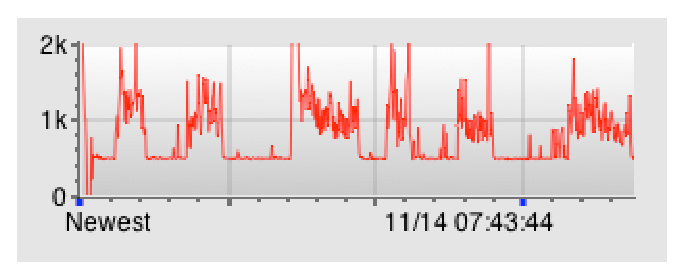
\includegraphics[width=5cm]{graphics/setup/Noise_Rate_Problem_cutout.eps}
   \caption[Muon modules' rate: noise problems]{Rate progression over the course of hours. Noticable raise in the cumulative rate of all panels in certain intervals}
  \end{figure}
  
  \begin{figure}
   \centering
   \includegraphics[width=0.9\textwidth]{graphics/setup/Histogram_noise_problem.eps}
   \caption[6 channel energy Histogram with noise]{Energy histogram of 6 channels, counts over ADC-Value. Two channels show a lot of noise around the peak position while four are developing into nice looking Landau Peaks}
  \end{figure}
  If the landau peaks were not identifiable due to prevalent electronic noise, the measurement was rendered useless as a lot of noise triggered events were recorded.
  As a countermeasure, in cooperation with Sascha Wuestling, potential equalisation by connecting the modules to the huge trough below the main spectrometer has been established. After the installation of the grounding, the peaking did not occur any more so the issue seems to be resolved. Now, one could make a start on setting gains, thresholds and acceleration voltages \ref{ch:Analysis:sec:GainsThresholdsAccVoltages}.
  
  %% ===========================
  \section{Gain-, Threshold and Acceleration Voltage Settings}
  \label{ch:Analysis:sec:GainsThresholdsAccVoltages}
  %% ===========================  
  
  A first amplification - linear with acceleration voltage - of the scintillation photons occurs in the photomultiplier tubes. As signals at first seemed too high for the DAQ to handle at nominal values of the datasheet, these were reduced to around \SI{1200}{\volt}. Now, the software gains and thresholds in the ORCA software needed to be set. 
    \begin{table}
    
    \centering
    \begin{tabular}{|l|cccccc|}
      \hline
      Panel/Side 	&1/A 	&1/B	&2/A	&2/B	&	&	\\
      \hline
      Card 	&3	&3	&3	&3	&	&	\\
      Channel	&0	&14	&3	&7	&	&	\\
      PMT Voltage	&1150	&1150	&1250	&1150	&	&	\\
      Threshold	&2110	&2110	&2110	&2110	&	&	\\
      Gains	&2350	&2400	&1200	&2850	&	&	\\
      \hline
      Panel/Side 	&3/A 	&3/B	&4/A	&4/B	&5/A	&5/B	\\
      \hline
      Card 	&6	&6	&6	&6	&6	&6	\\
      Channel	&0	&14	&3	&7	&	&	\\
      PMT Voltage	&1150	&1150	&1150	&1150	&1150	&1150   \\
      Threshold	&2110	&2110	&2110	&2110	&2110	&2110   \\
      Gains	&2450	&2400	&2150	&2550	&2100	&2400   \\
      \hline
      Panel/Side 	&6/A 	&6/B	&7/A	&7/B	&8/A	&8/B	\\
      \hline
      Card 	&9	&9	&9	&9	&9	&9	\\
      Channel	&0	&14	&3	&7	&	&	\\
      PMT Voltage	&1150	&1150	&1150	&1150	&1050	&1100	\\
      Threshold	&2110	&2110	&2110	&2110	&2110	&2110   \\
      Gains	&3400	&2100	&2400	&2500	&3950	&2900   \\
      \hline
    

   \end{tabular}
  \caption[Gains - thresholds - acceleration voltages]{{\bf Gains, thresholds and voltages:} These are the settings that appeared to be reasonable for each panel side; furthermore, the table displays the card and channel each side is associated with in the DAQ card system}
  \end{table}
  
  %% ===========================
  \section{Finding the best filter settings}
  \label{ch:Analysis:sec:Finding the best filter settings}
  %% ===========================  
  As the PMT tubes are directly, without any preamplifiers, connected to the DAQ, the signal lengths arriving at the latter are in the order of \SI{20}{\nano\second}. This poses a problem for filters as the sampling rates need to be high and anti-aliasing is inevitable. To find the best settings, a pulser has been set up to create events at known frequency and peak heigth. The pulser's signal form \todo{what form} was chosen as closely to the actual shape as possible, which is the "pin diode" form.
 
  \begin{figure}
	
\includegraphics[width = 0.9\textwidth]{graphics/dummy.eps}
	\caption[Pulser and signal shape]{Pulser shape on the left compared to actual signal shape on the right. }
  \end{figure}

  
  Now, to evaluate filter goodness, the width of the resulting energy histogram, which should, assuming perfect pulser signals and perfect filters, be monoenergetic, was analysed for each filter setting. This resulted in the following set of data:
  
  \begin{table}
	\caption[Energy resolution dependant on filter setting]{Energy resolution at different filter settings}
	\centering
	standard filter
	\begin{tabular}{c}
	\SI{50}{\nano\second} gap, \SI{0}{\second} shaping time\\
	
  	\begin{tabular}{ccc}
  		1& 2& 3\\
  		1& 2& 3\\
  		1& 2& 3\\
  		1& 2& 3\\
  	\end{tabular}
  	\end{tabular}\\
  	boxcar filter
  	\begin{tabular}{ccc}
  		1& 2& 3\\
  		1& 2& 3\\
  		1& 2& 3\\
  		1& 2& 3\\
  	\end{tabular}

  \end{table}
  On average, the boxcar filter at shaping lengths of \SI{150}{\nano\second} shows the most promising results, i.e. the sharpest peaks for any signal height. This concurs with the settings chosen for the active fpd veto; here slightly longer (around \SI{30}{\nano\second}) but comparable signals enter the DAQ, showing best results at the same filter settings\cite{KevinWierman}.
  That is why, for any measurements after \todo{run \& date}, the new filter settings were used, bringing up the need for new threshold and gain adaptions \ref{ch:Analysis:sec:GainsThresholdsAccVoltages}. 
  
  %% ===========================
  \section{Moun module's rates}
  \label{ch:Analysis:sec:Muon module's rates}
  %% ===========================  
  A simple first check into the data is possible simply by comparing the rates measured to literature values. Here, a flux of around 1 per \SI{}{\minute} and \SI{}{\square\centi\meter} through an area parallel to the ground is stated. Measured rates are in the order of \SI{250}{\hertz}. The muon modules' area is
  \begin{equation}
  	\SI{315}{\centi\meter} \cdot \SI{65}{\centi\meter} = \SI{2.05}{\square\meter}
  \end{equation}
  Considering the \SI{45}{\degree} tilt of the modules towards the horizontal, this area reduces to an effective area of 
  \begin{equation}
  	A_{\mathrm{eff}} = \sin{\left(\SI{45}{\degree}\right)} A_{\mathrm{real}} = \SI{1.45}{\square\meter}
  \end{equation}
  Further taking into account detection efficiencies $\eta$ discussed in \ref{ch:Analysis:sec:Module Efficiency}, we receive an estimation of effective rate of
  \begin{equation}
  	\Phi_{est} = \eta \frac{1}{\SI{}{\square\centi\meter}\SI{60}{\second}}A_{\mathrm{eff}} = \SI{225}{\hertz}
  \end{equation}
  It compares well to measured rates of \todo{calculate actual rates} ~ \SI{250}{\hertz}.
  
  %% ===========================
  \section{Modules in high magnetic fields}
  \label{ch:Analysis:sec:Modules in high magnetic fields}
  %% ===========================  
  For there is the need of moving the muon modules as close to the spectrometer tank as possible to register mostly muons that indeed went through the vessel, they are aligned closely to the air coil system. This brought up the problem of photomultiplier tubes having to work in high magnetic fields. Photomultipliers, as mentioned before, use electrons cascading in electric fields to generate amplified signals. Additional magnetic fields can keep the electrons from reaching the dynodes stopping the cascade thus keeping single events from being registered. As rate decreases strongly under these conditions \todo{are there runs showing that? ask nancy}, a solution needed to be found. As a simple, yet efficient passive counter measurement, a layer of mu-metal was wrapped around the modules. Mu-metal is a magnetically highly permeable material (here, $\mu_r\approx $\todo{find out permeability}) that guides the magnetic field lines inside itself. In doing so, the remaining flux inside a mu-metal surrounded volume, 
and with it the field strengths, drastically reduces.
  To test the improvement the mu metal coverage produces, measurements with rising aircoil currents have been performed.
  Steps in the size of tenths of the maximum current of mostly \SI{100}{\ampere}, in some cases only \SI{70}{\ampere}, were used to record rates over half an hour at each value.
  During the first run, due to a slow control problem, the current was not raised between two steps. Although displaying the expected behaviour - rates dropped much less than before - the measurement was repeated with the correct currents.
  Measurements show that the rate still drops at currents close to the maximum, though only to around \SI{90}{\percent} of initial values \ref{fig:aircoilCountsCurrent}. As, under normal measurement conditions, the coil currents are mostly around half the maximum value or less, the problem could be solved, as here, the reduction in rate is within the order errors' order.
  \begin{figure}

  \centering
  	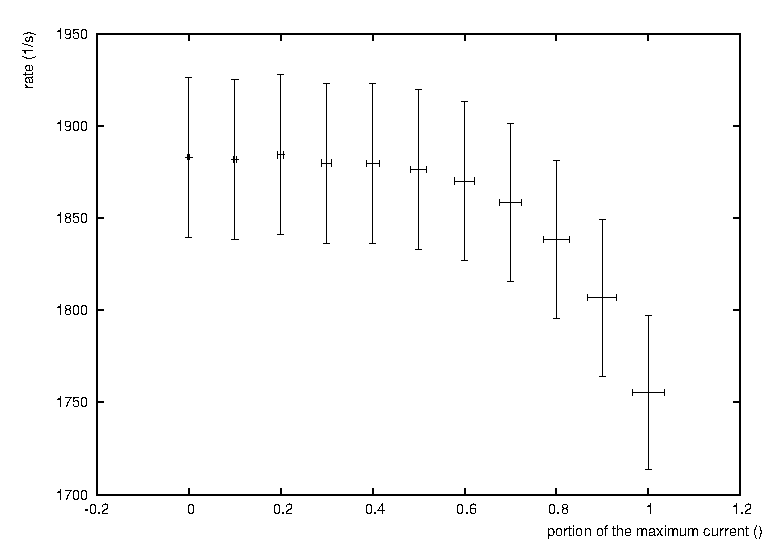
\includegraphics[width = 0.9 \textwidth]{graphics/aircoilCounts/aircoilsCountsCurrent.eps}
  	\caption[Rate dependance on magnetic fields]{Counts over air coil currents, with a maximum of \SI{100}{\ampere}. A clear decrease in rate is recognisable in the last 5 data points.}
  	\label{fig:aircoilCountsCurrent}
  \end{figure}
  

  %% ===========================
  \section{Module Stability}
  \label{ch:Analysis:sec:Module Stability}
  %% ===========================  
  If consistent factual statements on muon induced background are to be made, the modules need to work stable over the course of days, as rates are supposed to be comparable. For this reason, over the Christmas time 2012, a two-weekly measurement of half hourly runs has been taken, see \ref{tab:airCoilSettingsChristmas} for air coil settings used. Runs myo00000051 to myo00000675 contain the data of this measurement.
  \begin{table}
  \centering
   \begin{tabular}{|l|ccccccc|c|}
    \hline
    &&&&&&&&\\
    Coil \#	&1	&2	&3	&4	&5	&6	&7	&EMCS h	\\
    Current [A]	&10	&10	&14	&25	&42	&39	&54	&50  	\\
    &&&&&&&&\\
    Coil \# 	&8	&9	&10	&11	&12	&13	&14	&EMCS v	\\
    Current [A]	&54	&21	&36	&30	&21	&20	&56	&15    	\\
    &&&&&&&&\\
    \hline
   \end{tabular}
  \caption[LFCS settings stability measurement]{Runtime settings for air coils as proposed and for the comissionig measurements. These were kept static over the two weeks end 2012/beginning 2013}
  \label{tab:airCoilSettingsChristmas}
  \end{table}

  The time slot was chosen for the lowly frequented spectrometer hall's sake to minimise external impacts on data taking. For analysis, a simple program to count events in variable time bins was written, creating a count histogram for all the runs in the measurement period. The result can be seen in \ref{fig:moduleStability}. The observable fluctuation is well describable by fluctuations in atmospheric density, i.e. pressure and temperature, as ideally, air could be described by
  \begin{equation}
  	\rho = \frac{R}{M}\frac{p}{T}
  \end{equation}
  where $\rho$ is the density, R is the gas constant, M is the molar mass of air and p and T are pressure and temperature respectively.
  If one looks at the data from \todo{find weather station data, see if it fits fluctuations, maybe cascade data to back it up?}
  \begin{figure}
	\centering
  	
\includegraphics[width = 0.9 \textwidth]{graphics/dummy.eps}
  	\caption[Atmospheric density stability measurement]{Atmospheric density as a function of time over the course of two weeks the muon measurements took place. Note the }
  	\label{fig:moduleStability}
  \end{figure}

  %% ===========================
  \section{Module Efficiency}
  \label{ch:Analysis:sec:Module Efficiency}
  %% ===========================  
  The runs used for stability measurements, as well as any other run including modules six, seven and eight, can be used to check muon module seven for efficiency. For tests on other modules, the geometry would need to be changed so that the one to be checked is in between at least two other modules.
  For analysis, the function determineEfficiency() \ref{ch:Analysis software:sec:methods of the class run:subsec:determineEfficiency}
  has been written.
  The principle is the following: considering the small change in momentum direction high energy muons achieve through interaction with matter, one can assume straight-lined paths. From that follows, that if two parallel planes, that can be used to describe the scintillating volumes, are hit, any other, also parallel plane, in between those two will be hit as well. Keeping this in mind, one can analyse data for events registered in both modules 6 and 8 and cross check whether a event has been detected in module 7 as well. The quota of events in all three modules compared to those detected in 6 and 8 - but including the triple events - shows the efficiency of module 7.
  It shows that during the measurement period end of 2012, the efficiencies were at \todo{rerun} \SI{94 }{\percent} which is less than one would expect at a scintillator thickness of \SI{5}{\centi\meter} for muons perpendicular to the largest module surface, even more for any other.
  For that reason, the filter settings were checked and changed to the boxcar filter with a gap of 150 ns from the before used \todo{exact name} filter. However, the expected efficiency increase was not observable, the average efficiencies before and after are within the margin of error of the other.
  To examine the problem further, another idea came up: modules 3, 4 and 5, that are located next to each other could be used for efficiency measurements as well considering theiy are stacked in an upright way. Using the program on those three modules resulted in even lower efficiencies of \SI{50(3)}{\percent}. This raises the question wheter this is not an effect of signal filtering, but a previously not considered physics effect. One thing comming to mind is deviation of the muon track from linear forms. This feature would comply with the seemingly lower efficiency at the upright stacked modules, where, at equal bending radii, the ratio of muons travelling around the middle module is higher due to the lower total area in stacking direction.
  This thesis should be tested. This can be done both by simulating the cosmic muons including magentic fields and empirically by varying the distance between teh single modules. The latter is difficult not only because the modules are heavy and not made for lifting (no designated carrying structures), but also because movement always means potential danger to the photomultiplier tubes and their connection to the scintillators.
  Furthermore, if all coils and solenoids were to be turned of simultaneously at some point, one could collect data then and see how efficicencies change during that (there have been runs taken when that was still the case, but only few modules were working properly at that point).
  If the dependence on module distance turns out to be true, but the efficiencies are still below expected values at the lowest possible distances, a possible improvement would be to use preamplifiers before signals arrive at the DAQ. These would widen the signals timewise leading to a more easily detectable signal for the filters.
  
  %% ===========================
  \section{Photo Multiplier Tube Test with Sr source}
  \label{ch:Analysis:sec:PhotoMultiplierTests}
  %% ===========================
  
  With sets of four photomultiplier tubes being read out over one cable, and, consequently, via one channel, the test of individual PMTs is not trivial. Nevertheless, a method using a \SI{}{\mega\becquerel} $\rm ^{90}Sr$ source to trigger events was used to check functionality. Of course, all tubes were able to see the source at any position but rates were expected to rise as the distance to any of the tubes shrank. A source holder was constructed from acrylic glass to shield the user from radiation and to attach the source to the modules, as a large dependence of rate on the position was found when the source was simply duct taped to the modules. As the foil mantling of the modules absorbs a non negligible part of the radiation emitted from the source, it had to be ensured that the number of layers was equal for all measurements. This was given only below the modules as the foil has been folded around them at the ends in a gift wrapping way. Thus, the source was pretty far away from the photomultiplier 
tubes making it more difficult to distinguish between them. A first measurement was then to check for exactly that distinguishability.\todo{insert measurement for small steps over PMTs positions}.
  \begin{figure}
  	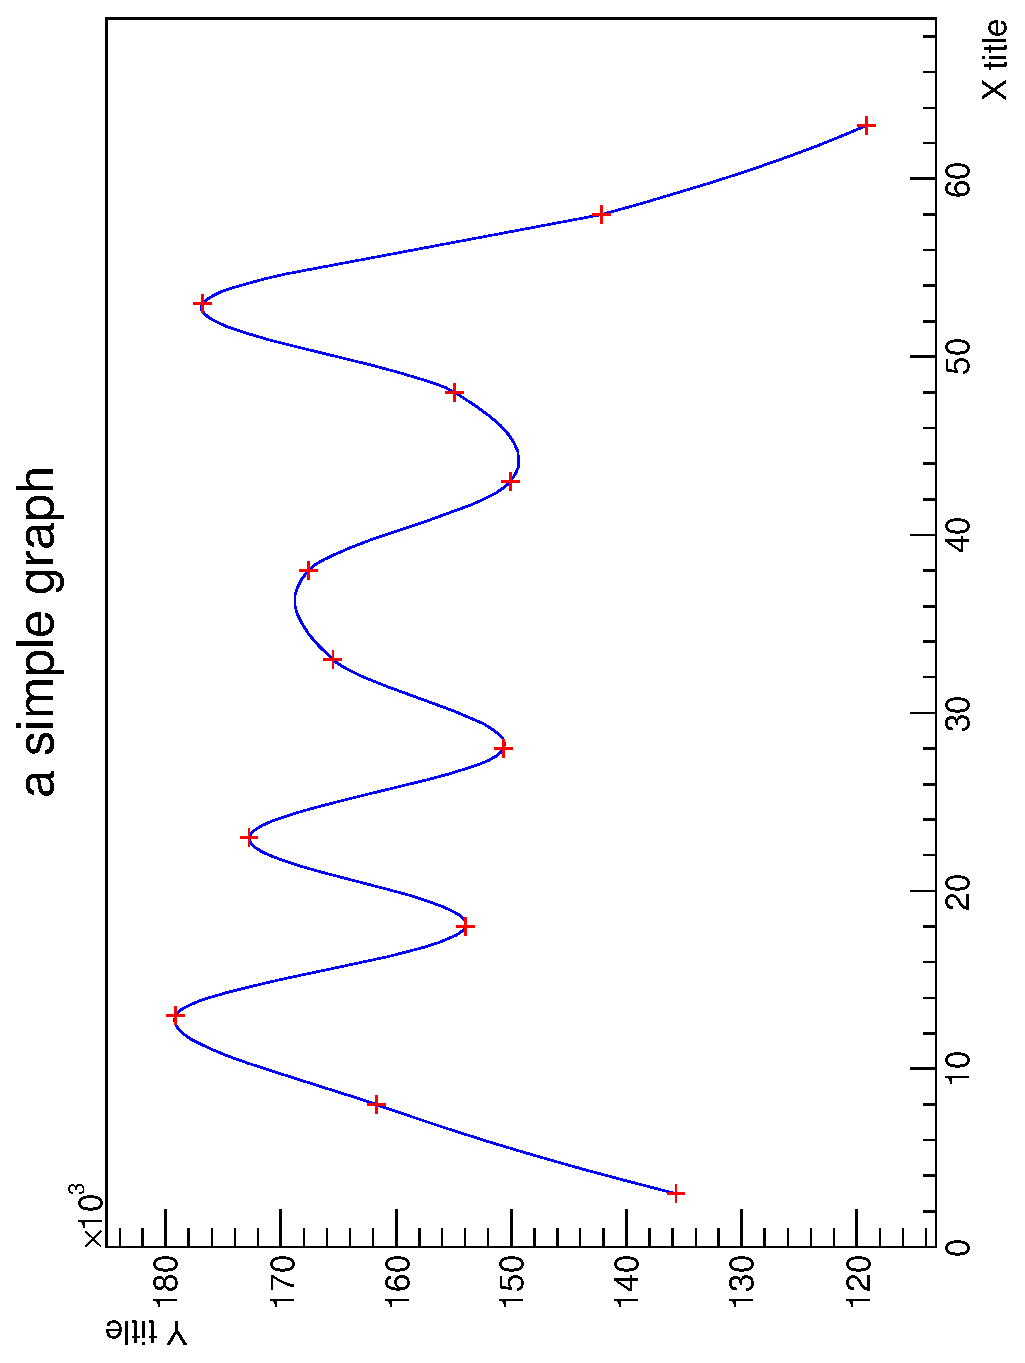
\includegraphics[angle = -90, width = 0.9 \textwidth]{graphics/cobalt/876_parallel_good.eps}
  	\caption[Rate scanning with cobalt source]{}
  \end{figure}

  \begin{figure}
  \centering
  	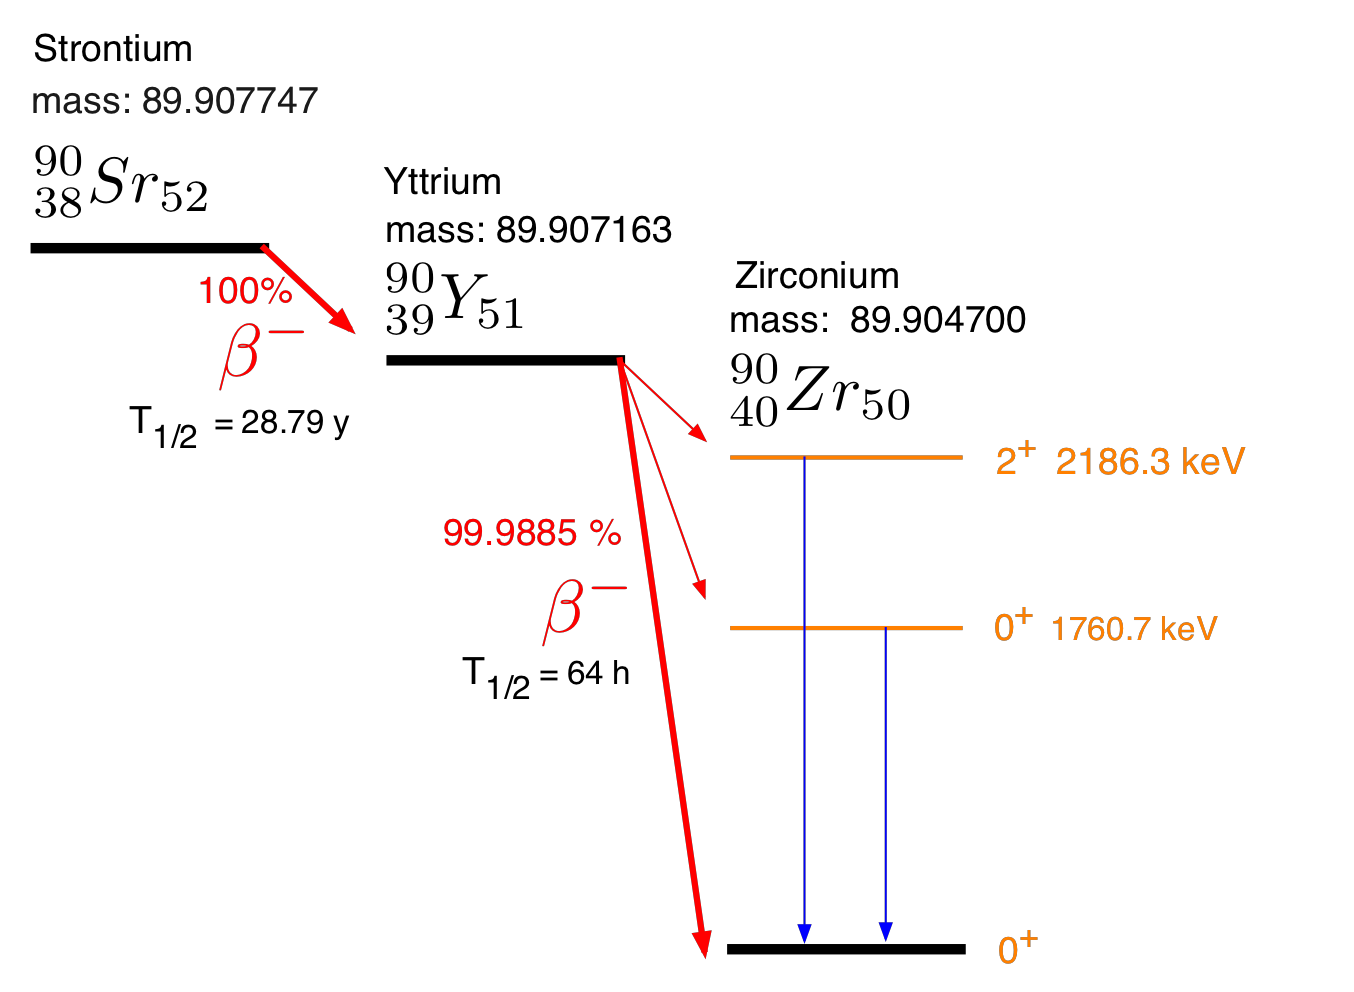
\includegraphics[width = 0.5 \textwidth]{graphics/cobalt/Sr90_decay.eps}
  	\caption[Cobalt decay mechanisms]{Decay mechanism of $^{90}$Sr: first a lower ernergetic decay to $^{90}$Y emitting \SI{544}{\kilo\electronvolt}/\SI{}{\square c} electrons, from that most probably a higher energetic decay to $^{90}$Zr ground state (\SI{2.29}{\mega\electronvolt}/\SI{}{\square c} electrons) or, with low probabilty, to one of two of its excited states.}
  \end{figure}

  As one can see a rise in rate at the positions the tubes are located at, it was decided that four measurements per module and side were sufficient, especially as all measurements can afterwards be compared to each other.
  The tube positions at \todo{n,n,n,n cm} were used as measurement positions as well. For each side, a run has been taken containing five minute subruns for every position. Figure \ref{fig:SrRatesPMT} shows the result of these measurements. One can see that the gerneral shape of each side compares very well to the others. Exceptions are \todo{which ones different?}showing slight, but acceptable deviations off the norm.
  \begin{figure}
	\centering
	%\label{fig:CoRatesPMT}
 	\begin{minipage}[d]{0.24 \textwidth}
		  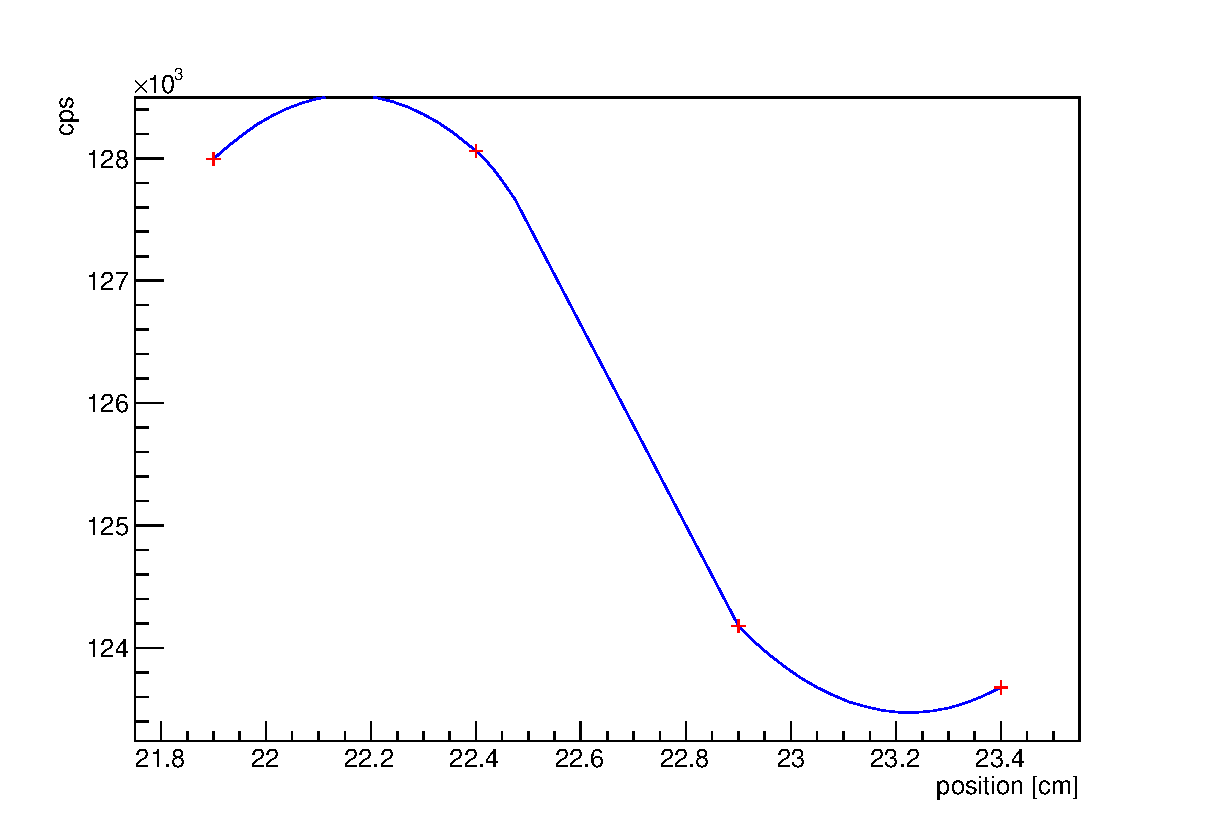
\includegraphics[width=\textwidth]{graphics/cobalt/modules/1A.eps}
	\end{minipage}
	\begin{minipage}[d]{0.24 \textwidth}
		  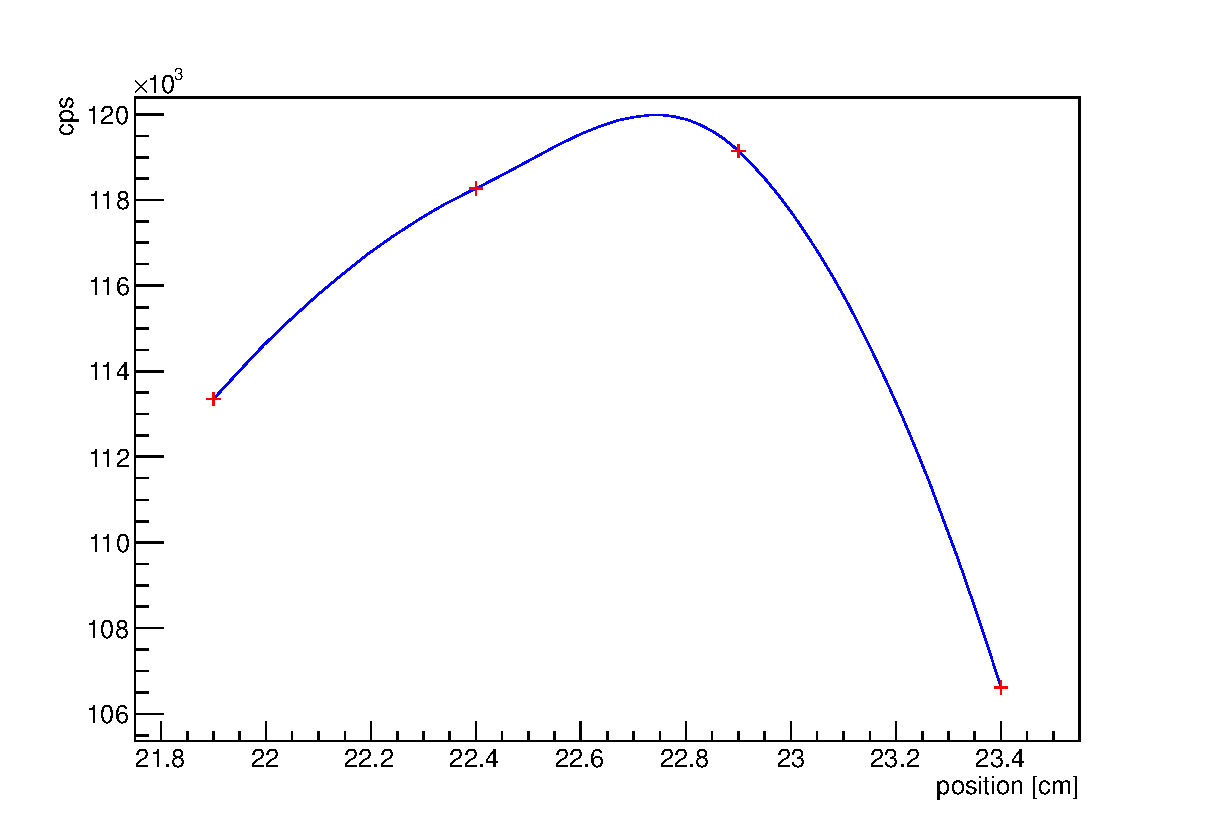
\includegraphics[width=\textwidth]{graphics/cobalt/modules/1B.eps}
	\end{minipage}
	\begin{minipage}[d]{0.24 \textwidth}
		  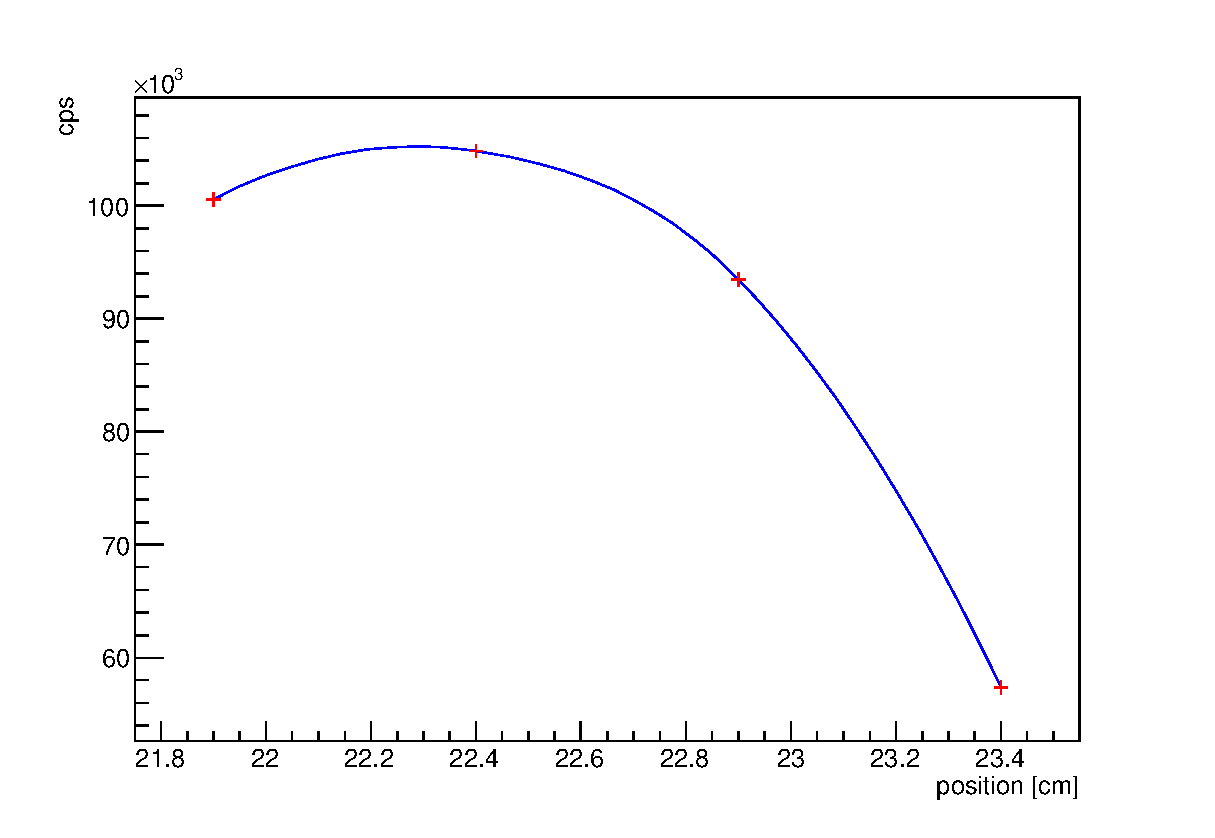
\includegraphics[width=\textwidth]{graphics/cobalt/modules/2A.eps}
	\end{minipage}
	\begin{minipage}[d]{0.24 \textwidth}
		  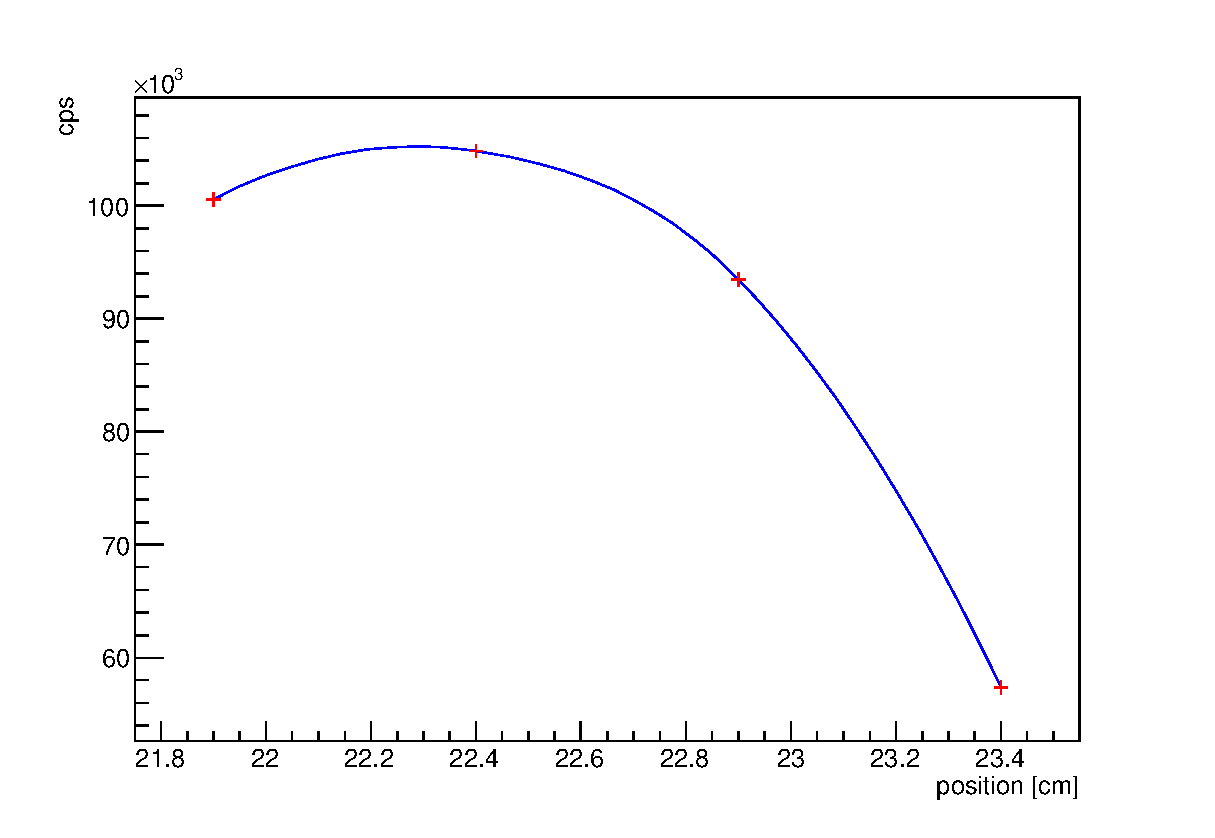
\includegraphics[width=\textwidth]{graphics/cobalt/modules/2A.eps}
		  %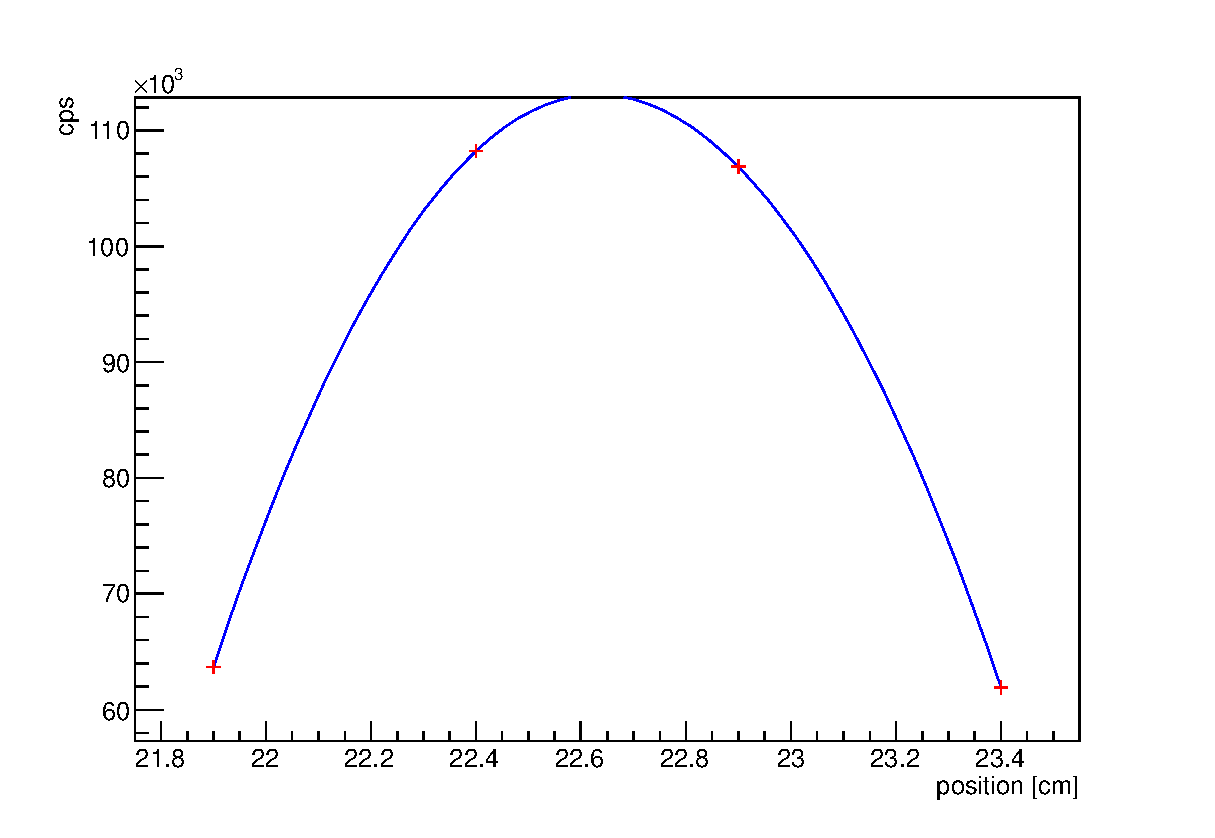
\includegraphics[width=\textwidth]{graphics/cobalt/modules/2B.eps}
	\end{minipage}\newline
	
	\begin{minipage}[d]{0.24 \textwidth}
		  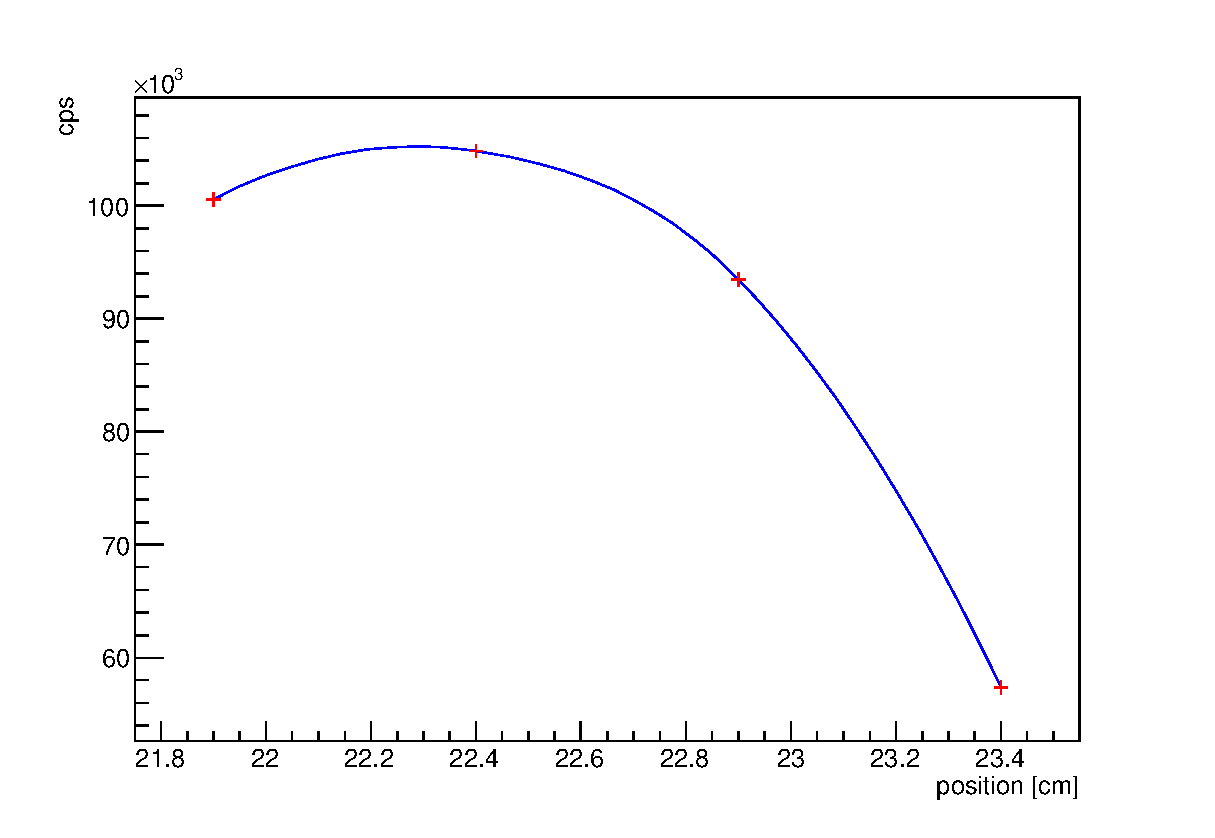
\includegraphics[width=\textwidth]{graphics/cobalt/modules/2A.eps}
		  %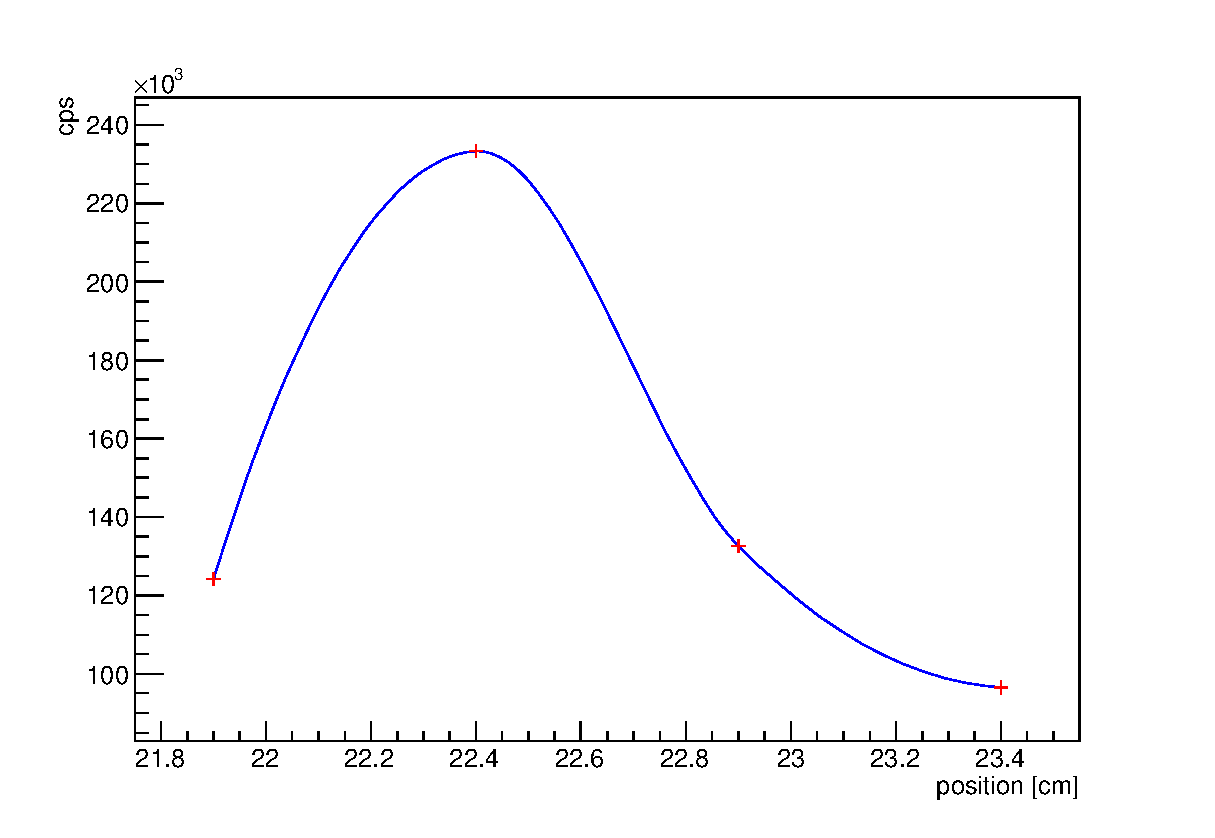
\includegraphics[width=\textwidth]{graphics/cobalt/modules/3A.eps}
	\end{minipage}
\begin{minipage}[d]{0.24 \textwidth}
		  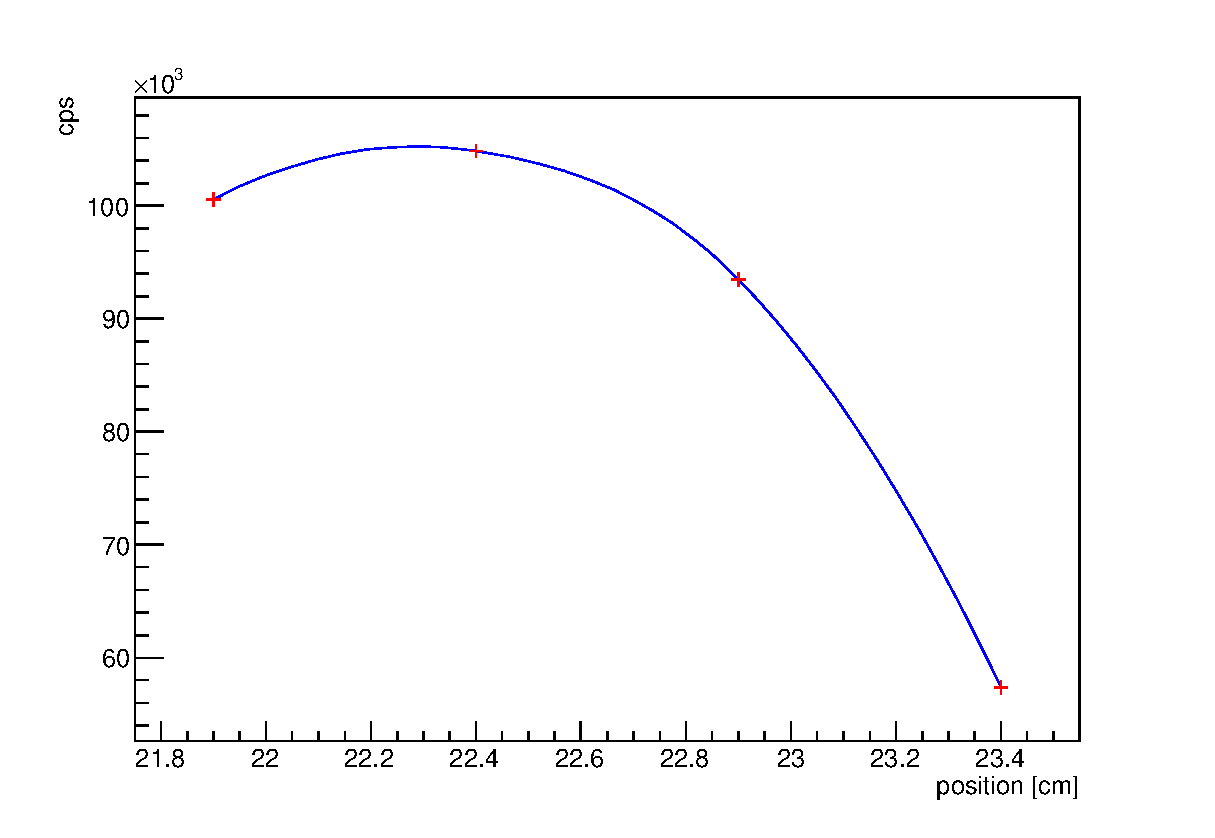
\includegraphics[width=\textwidth]{graphics/cobalt/modules/2A.eps}
		  %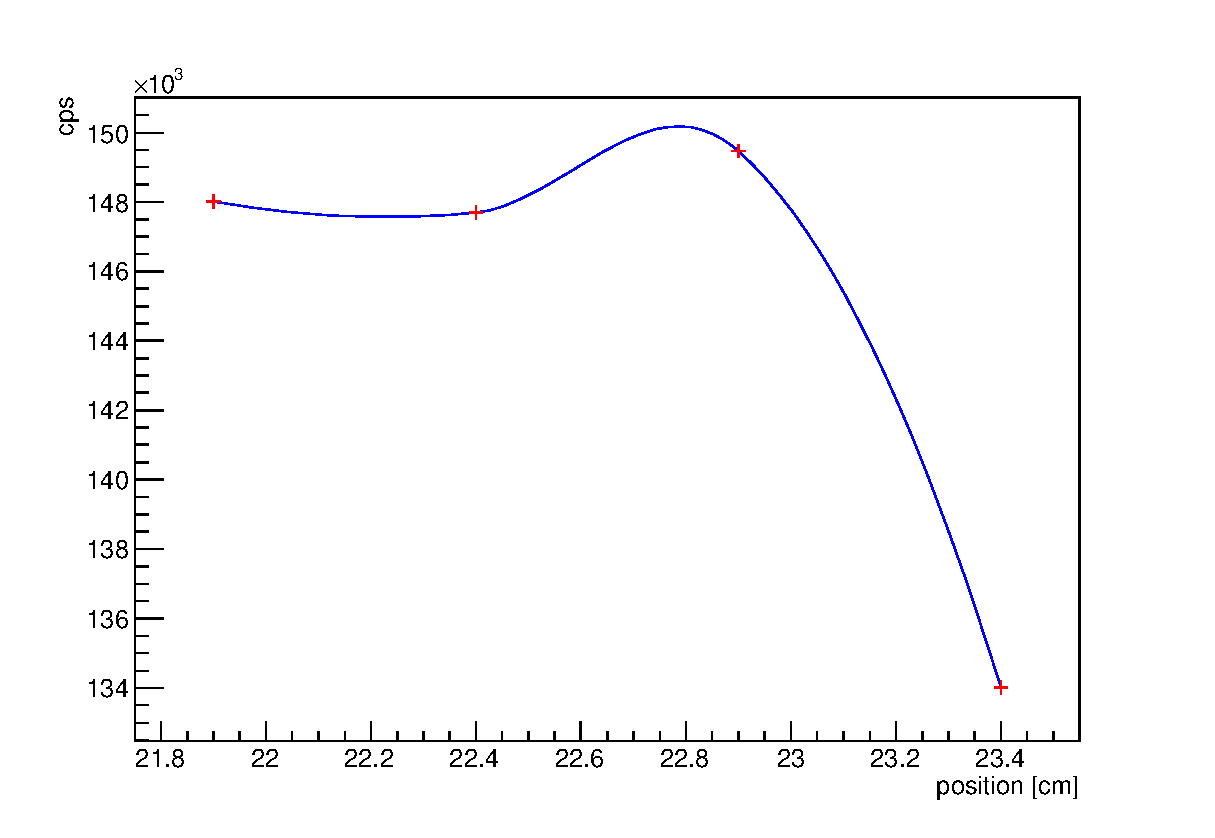
\includegraphics[width=\textwidth]{graphics/cobalt/modules/3B.eps}
	\end{minipage}
	\begin{minipage}[d]{0.24 \textwidth}
		  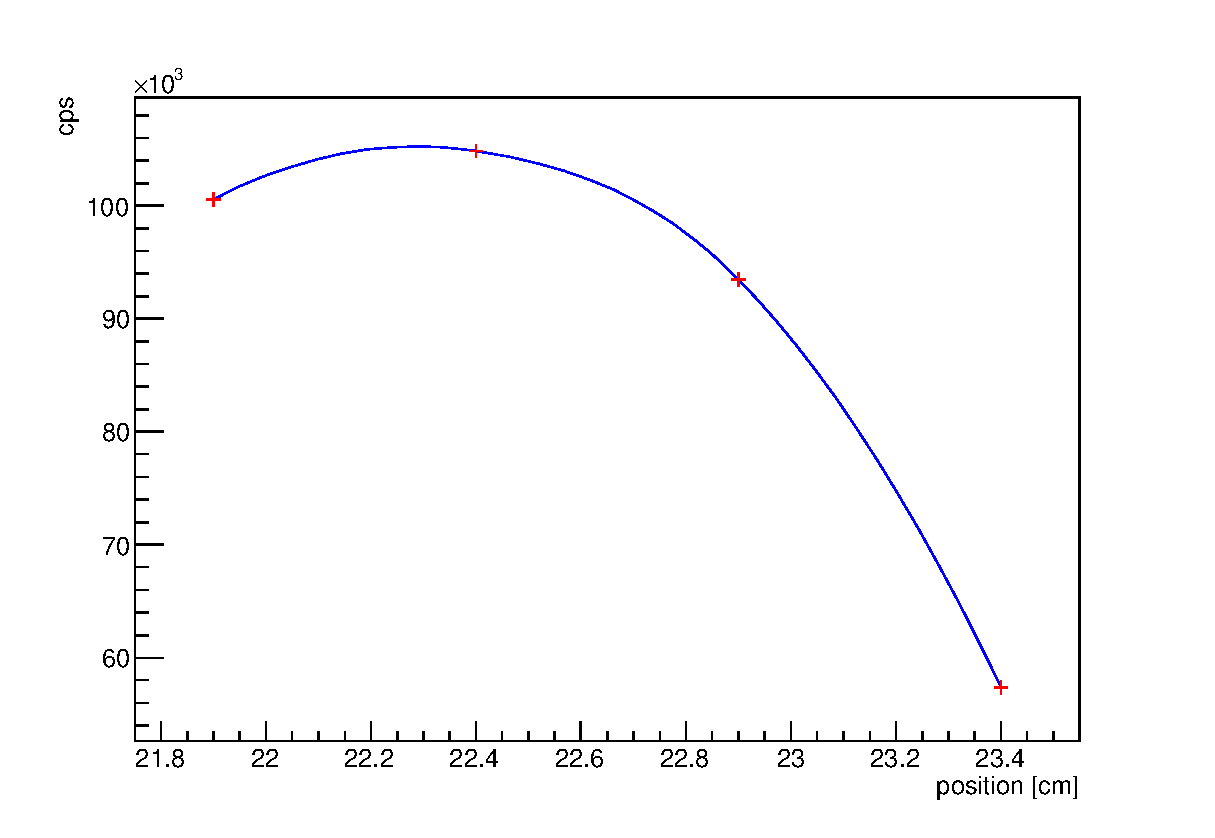
\includegraphics[width=\textwidth]{graphics/cobalt/modules/2A.eps}
		  %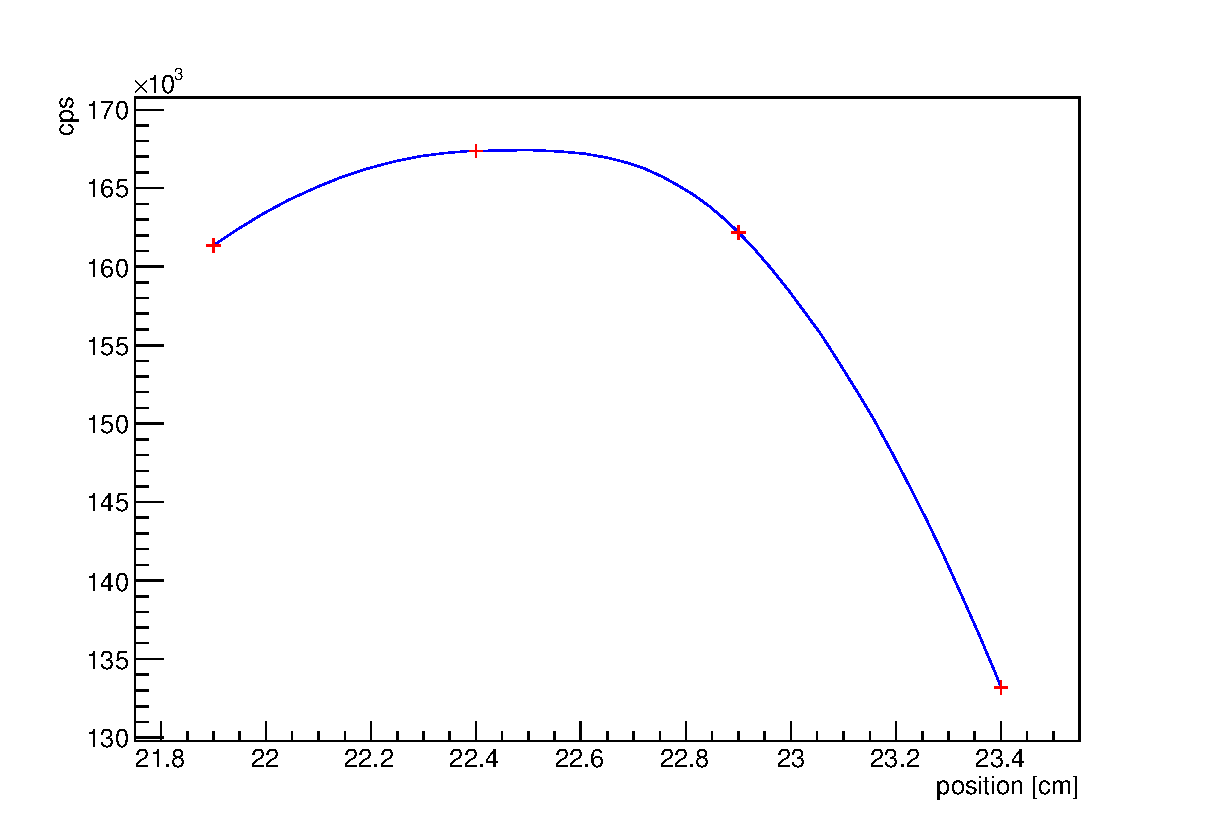
\includegraphics[width=\textwidth]{graphics/cobalt/modules/4A.eps}
	\end{minipage}
	\begin{minipage}[d]{0.24 \textwidth}
		  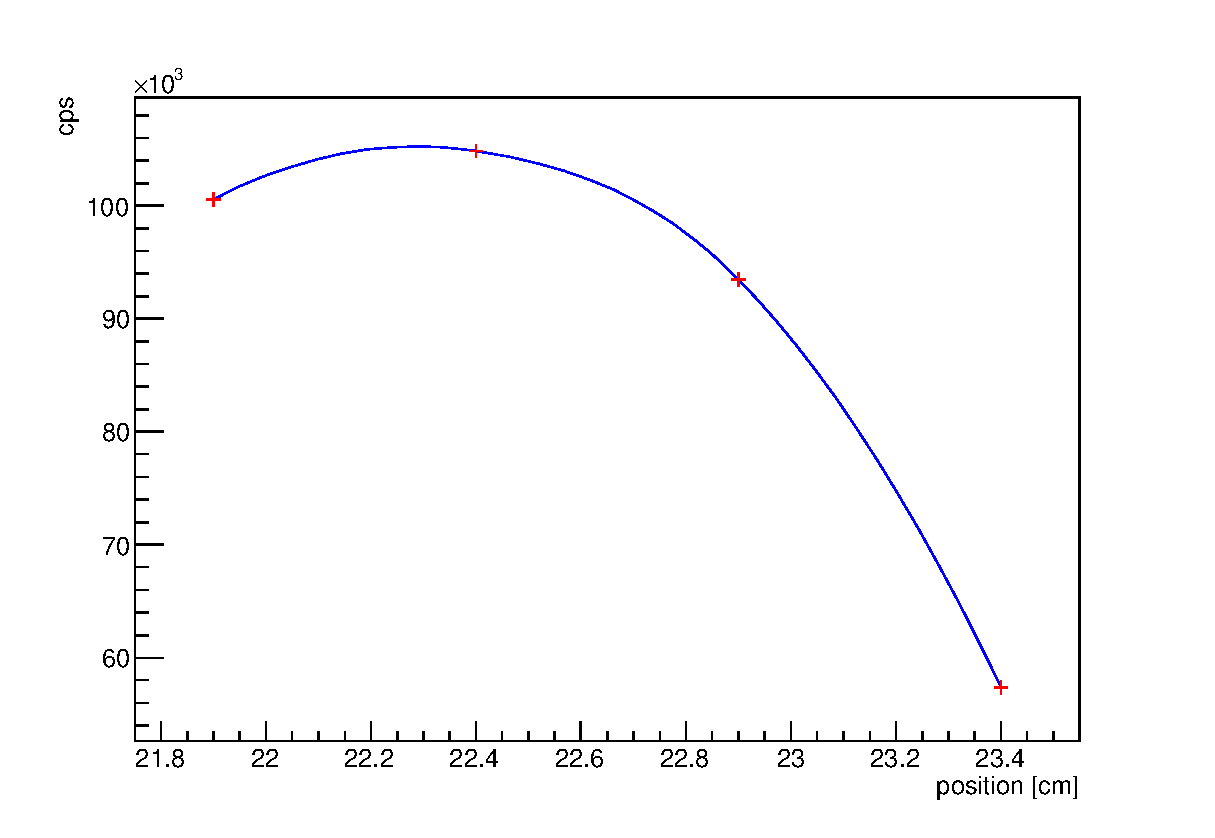
\includegraphics[width=\textwidth]{graphics/cobalt/modules/2A.eps}
		  %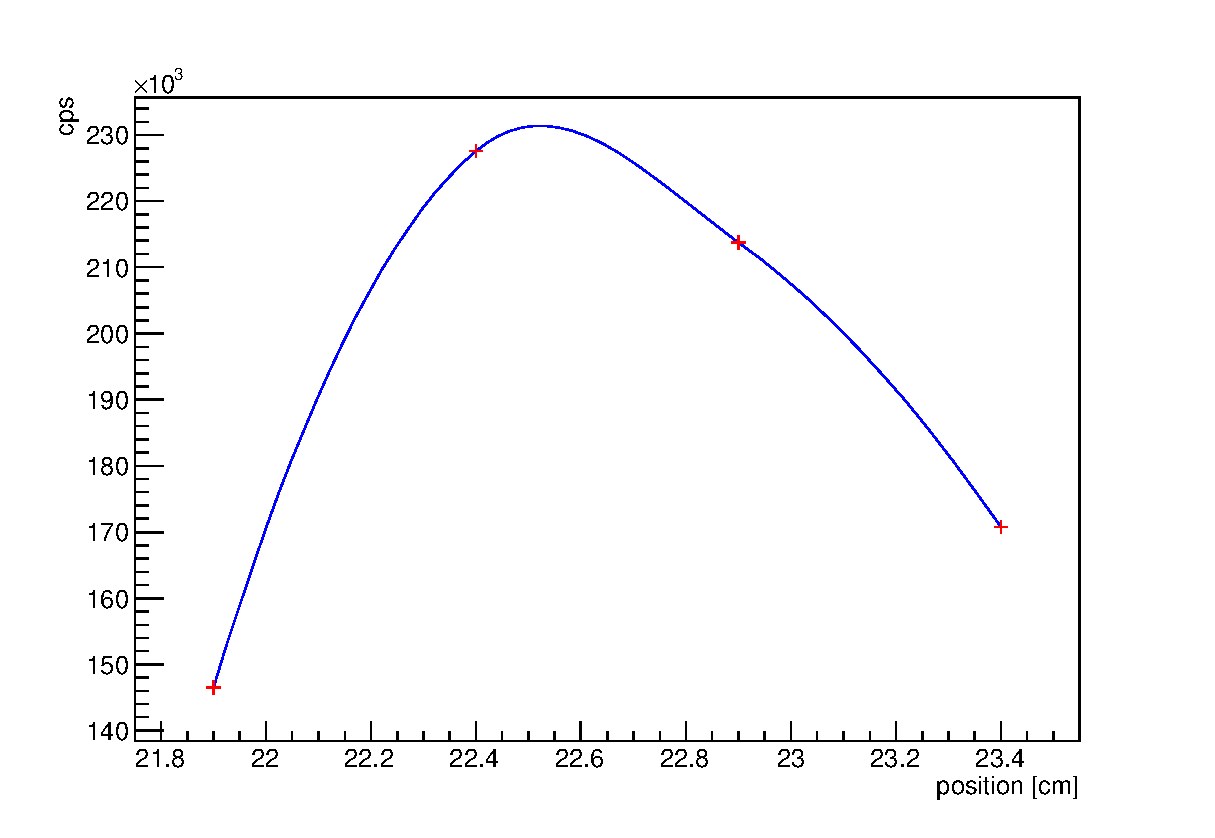
\includegraphics[width=\textwidth]{graphics/cobalt/modules/4B.eps}
	\end{minipage}\newline
	
	\begin{minipage}[d]{0.24 \textwidth}
		  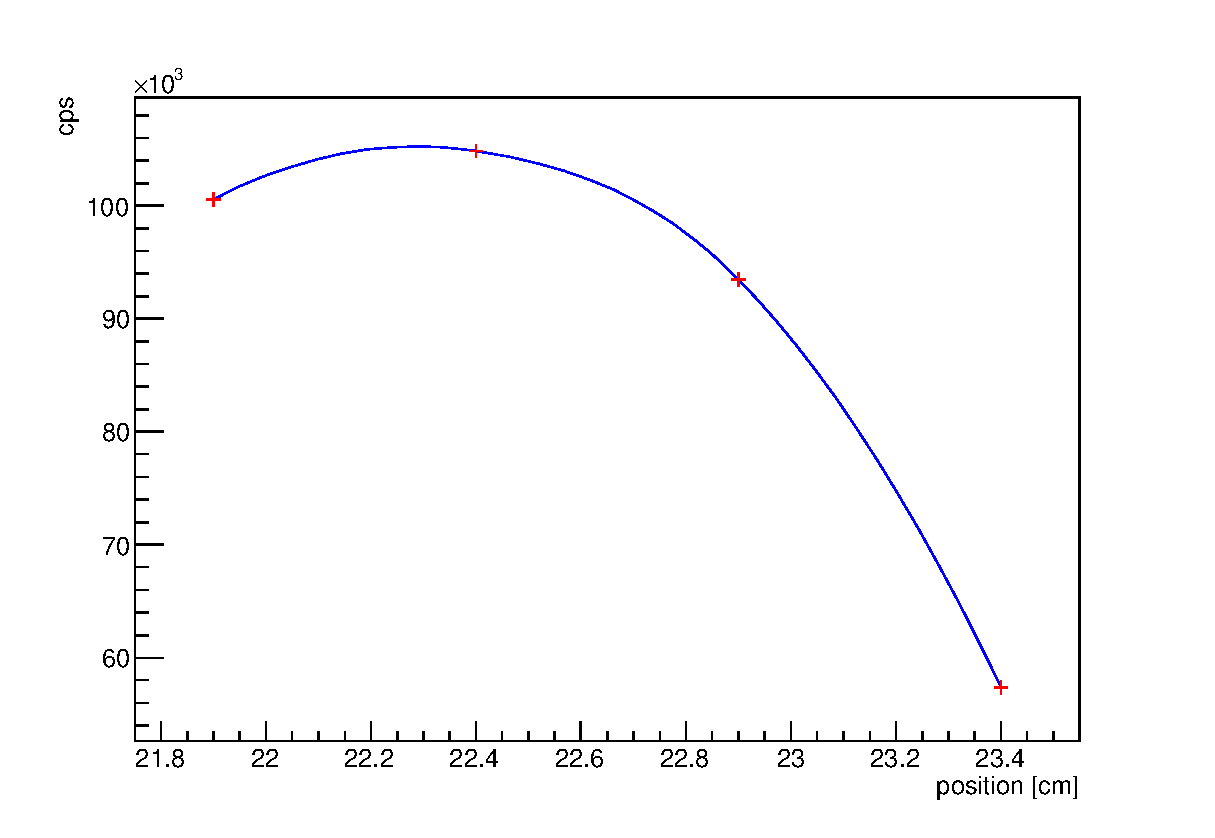
\includegraphics[width=\textwidth]{graphics/cobalt/modules/2A.eps}
		  %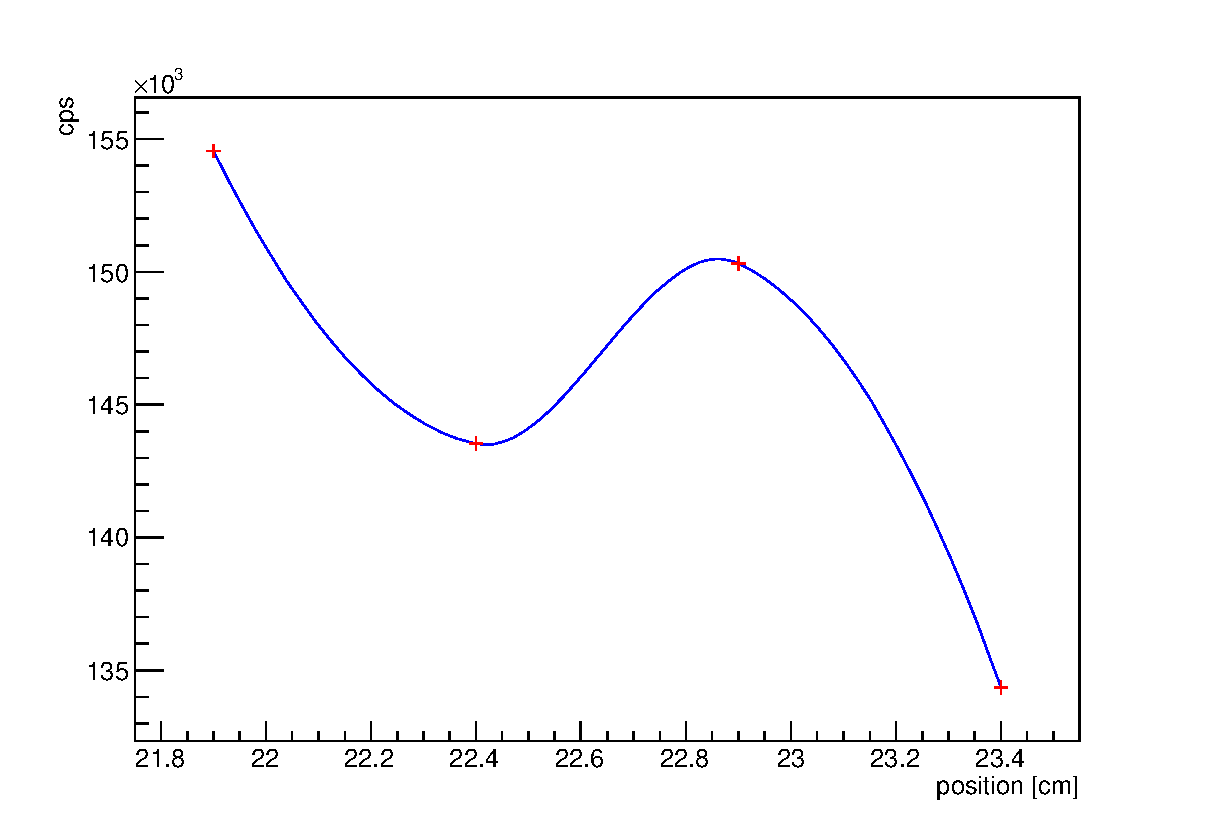
\includegraphics[width=\textwidth]{graphics/cobalt/modules/5A.eps}
	\end{minipage}
	\begin{minipage}[d]{0.24 \textwidth}
		  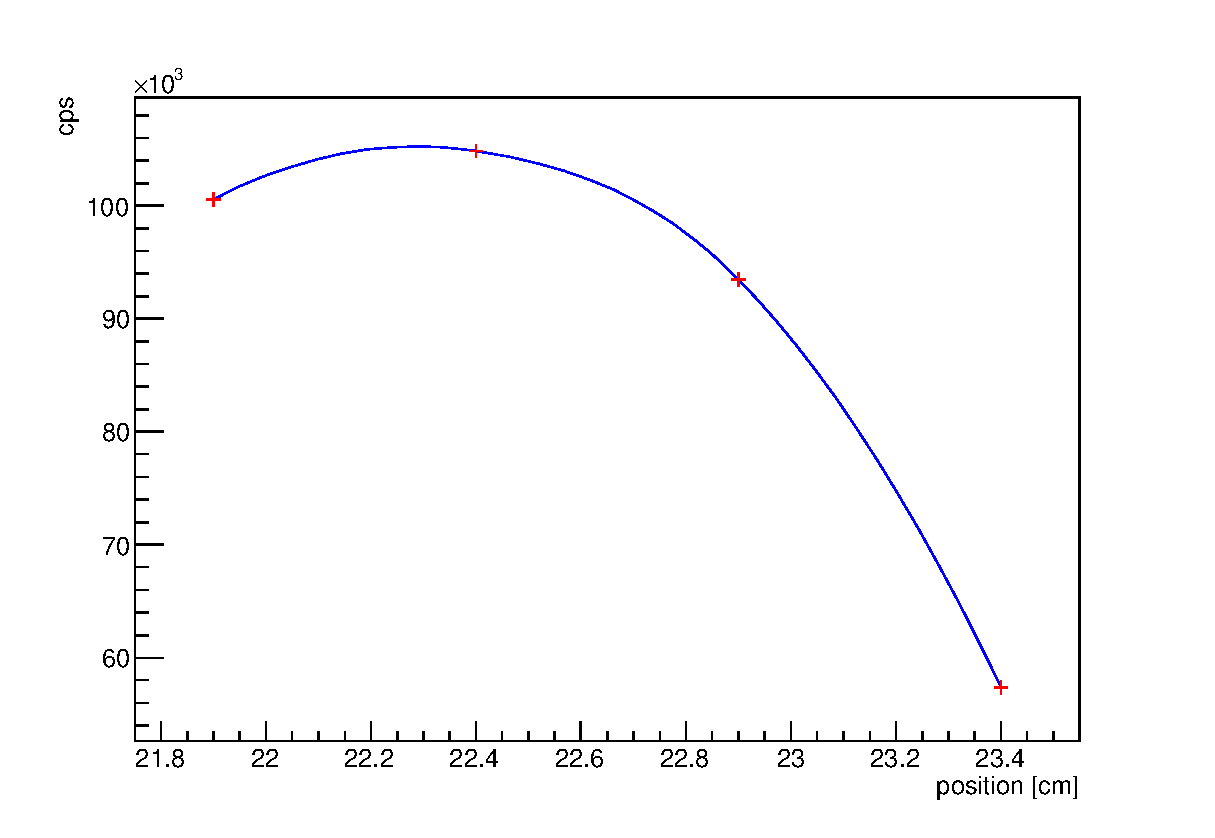
\includegraphics[width=\textwidth]{graphics/cobalt/modules/2A.eps}
		  %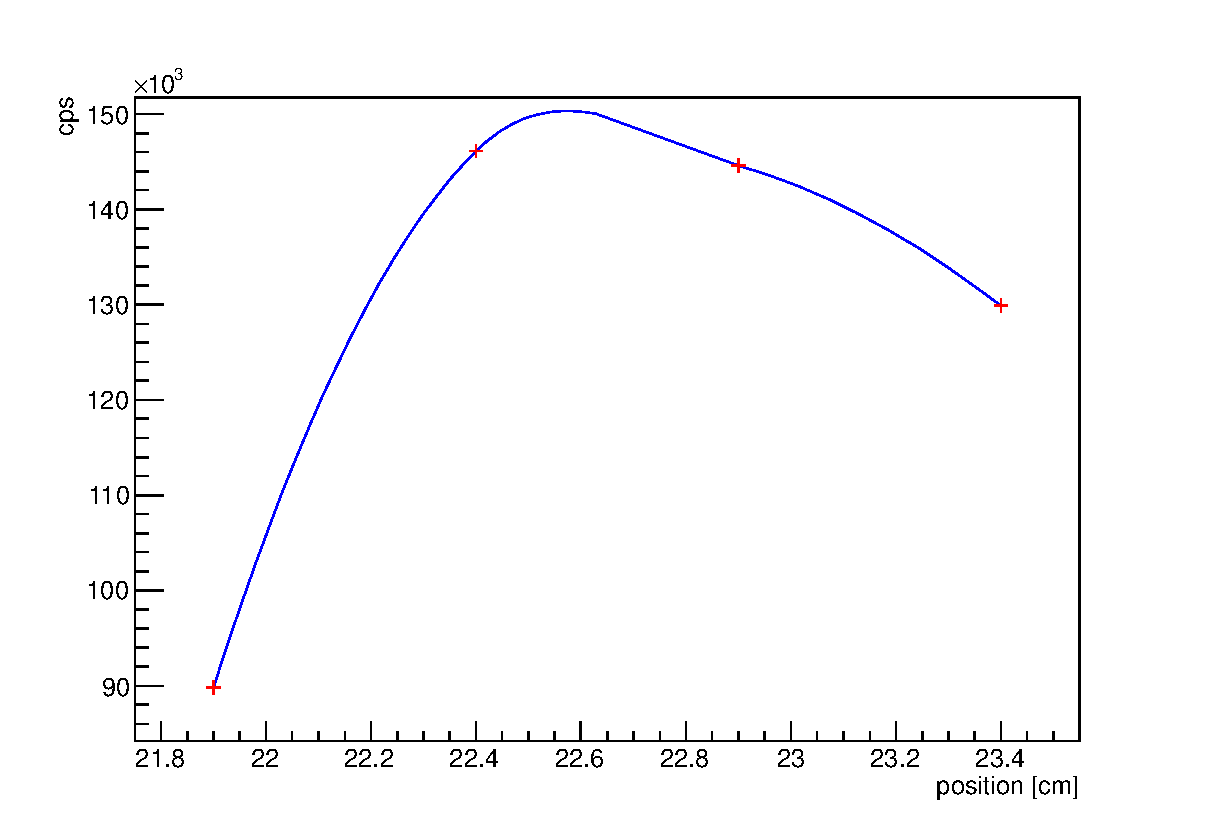
\includegraphics[width=\textwidth]{graphics/cobalt/modules/5B.eps}
	\end{minipage}
	\begin{minipage}[d]{0.24 \textwidth}
		  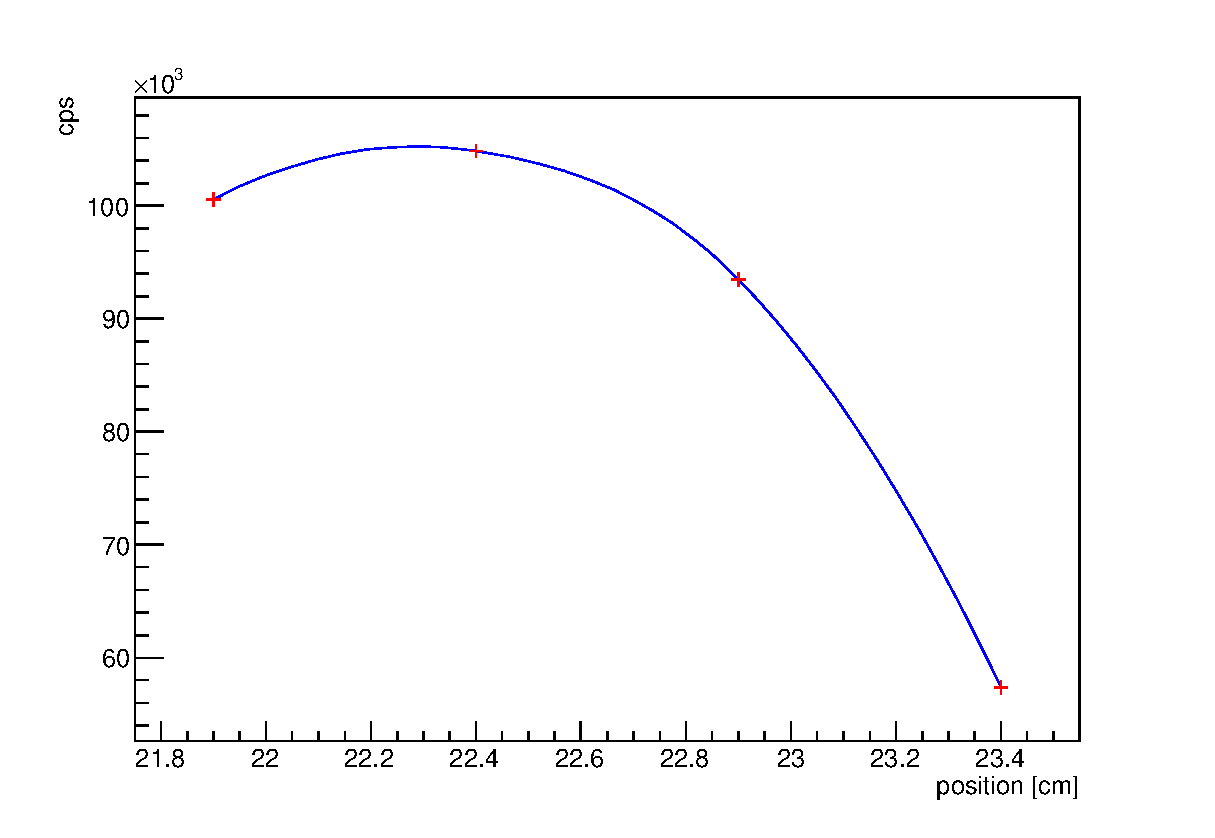
\includegraphics[width=\textwidth]{graphics/cobalt/modules/6A.eps}
	\end{minipage}
	\begin{minipage}[d]{0.24 \textwidth}
		  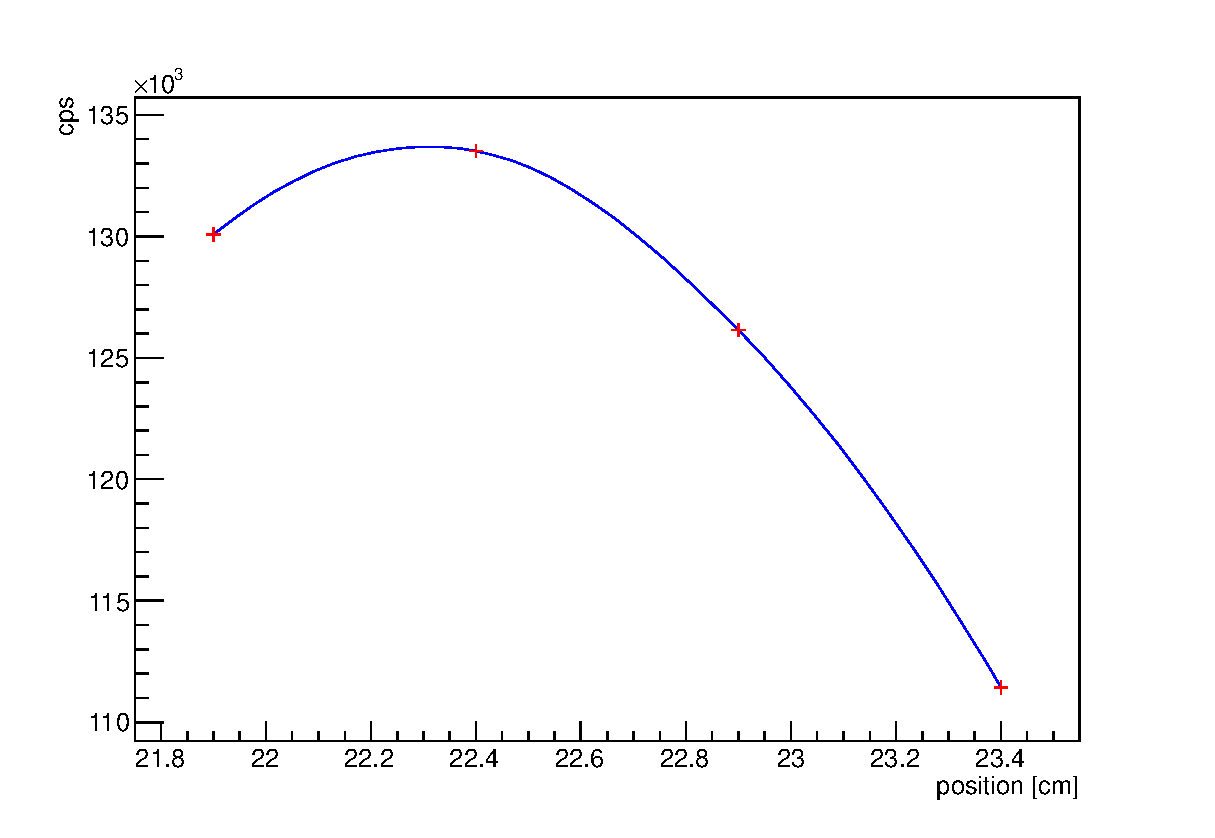
\includegraphics[width=\textwidth]{graphics/cobalt/modules/6B.eps}
	\end{minipage}\newline
	
	\begin{minipage}[d]{0.24 \textwidth}
		  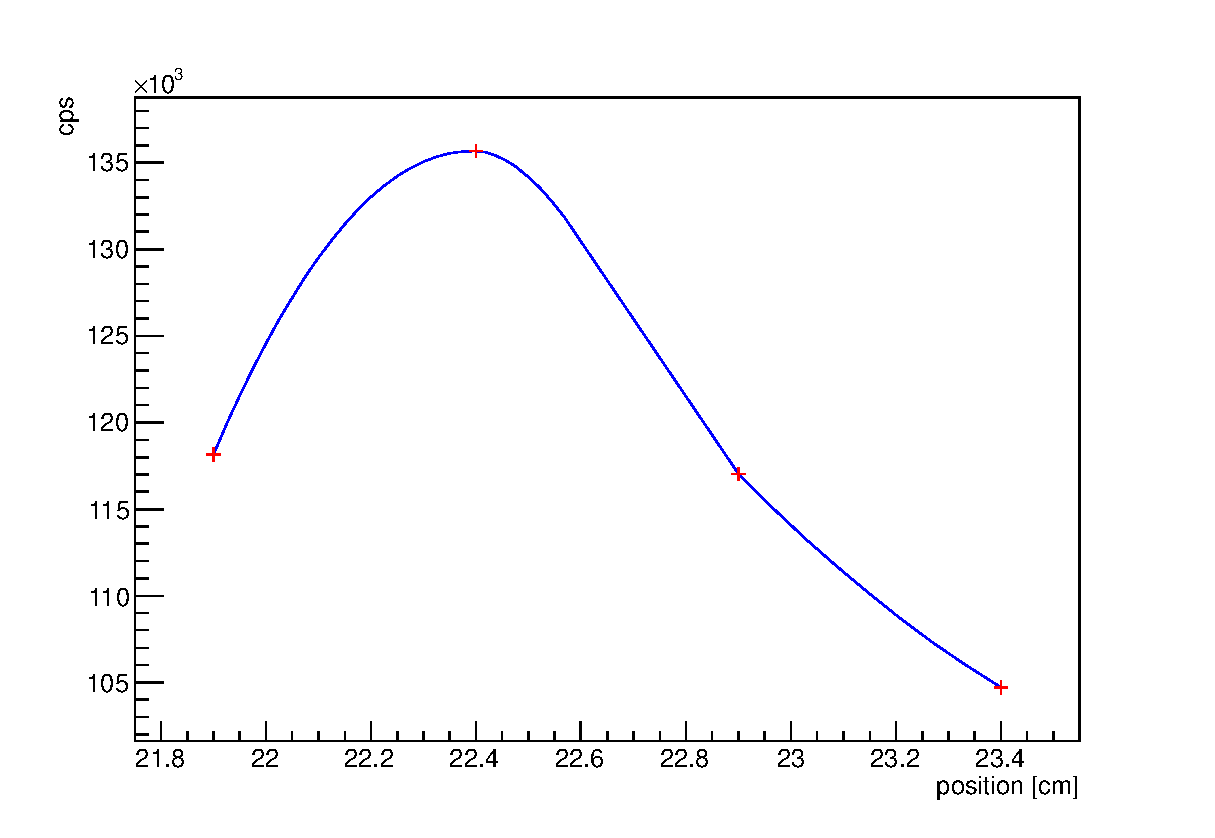
\includegraphics[width=\textwidth]{graphics/cobalt/modules/7A.eps}
	\end{minipage}
	\begin{minipage}[d]{0.24 \textwidth}
		  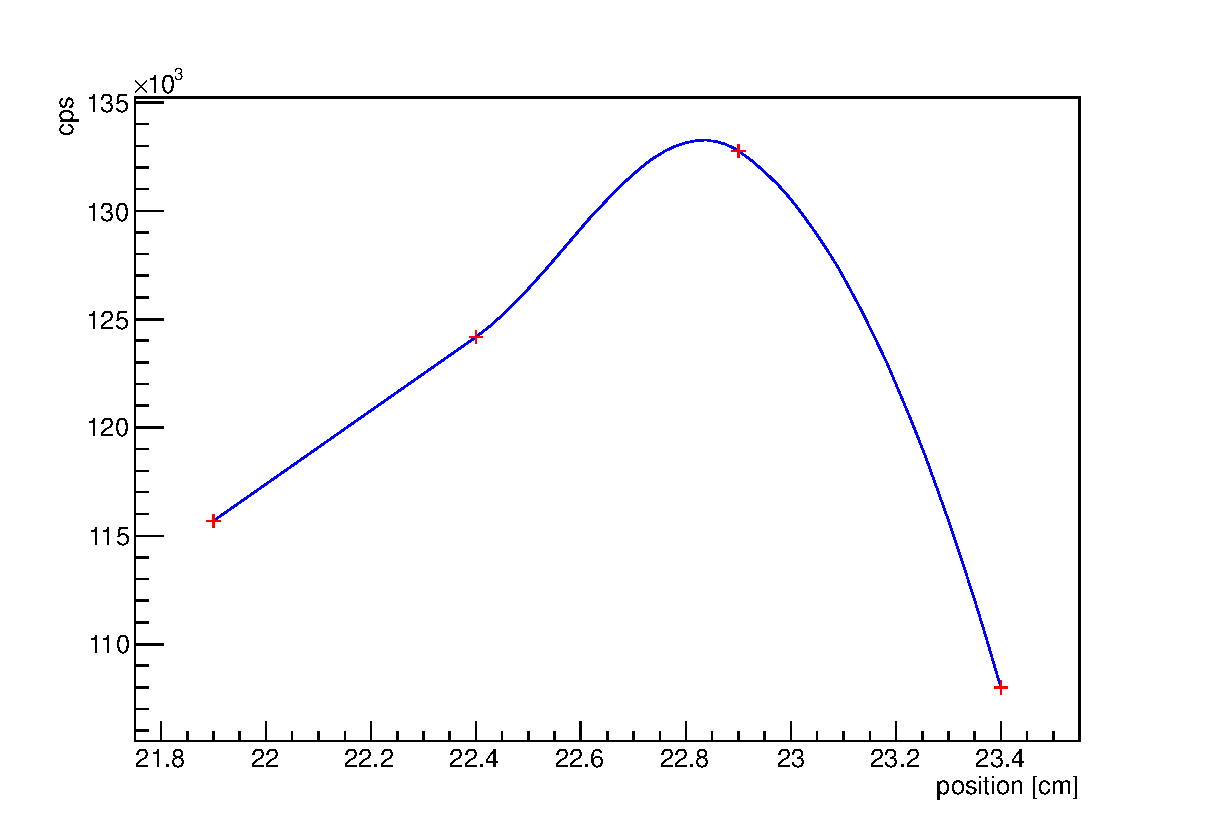
\includegraphics[width=\textwidth]{graphics/cobalt/modules/7B.eps}
	\end{minipage}
	\begin{minipage}[d]{0.24 \textwidth}
		  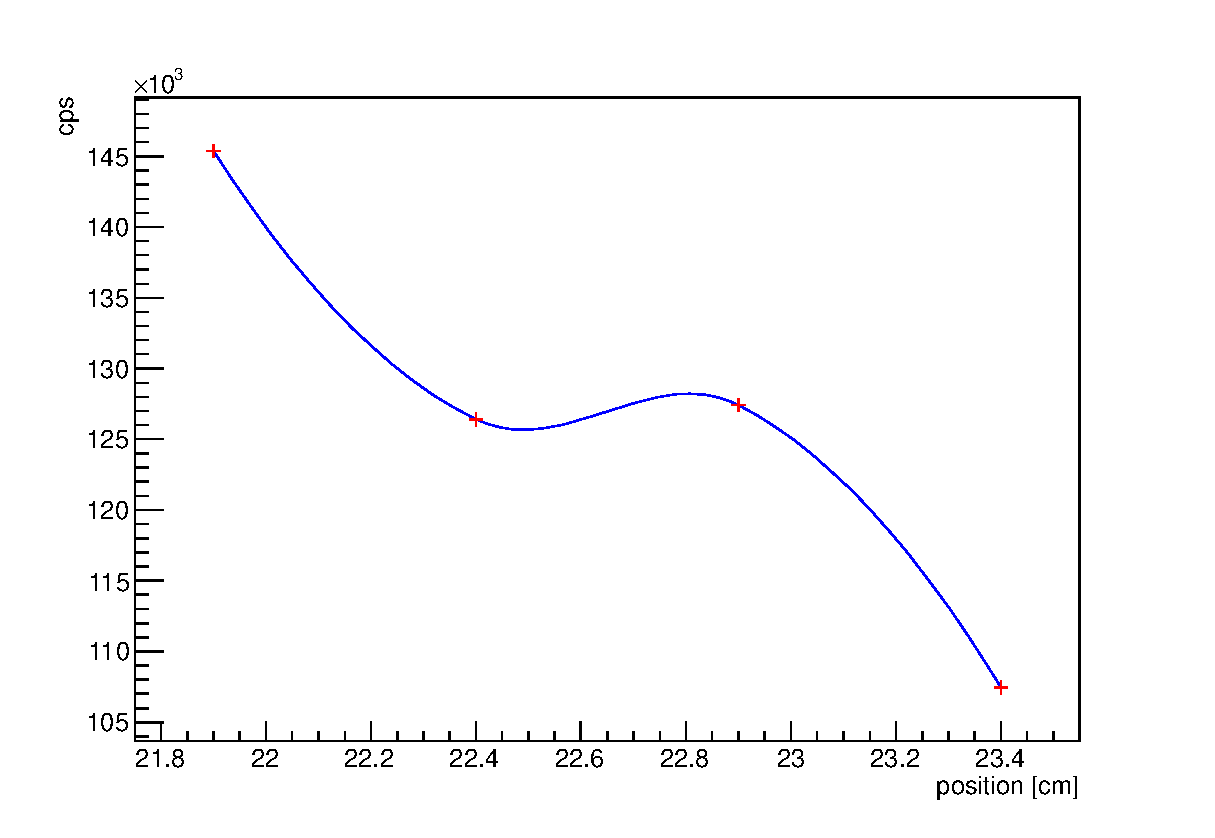
\includegraphics[width=\textwidth]{graphics/cobalt/modules/8A.eps}
	\end{minipage}
	\begin{minipage}[d]{0.24 \textwidth}
		  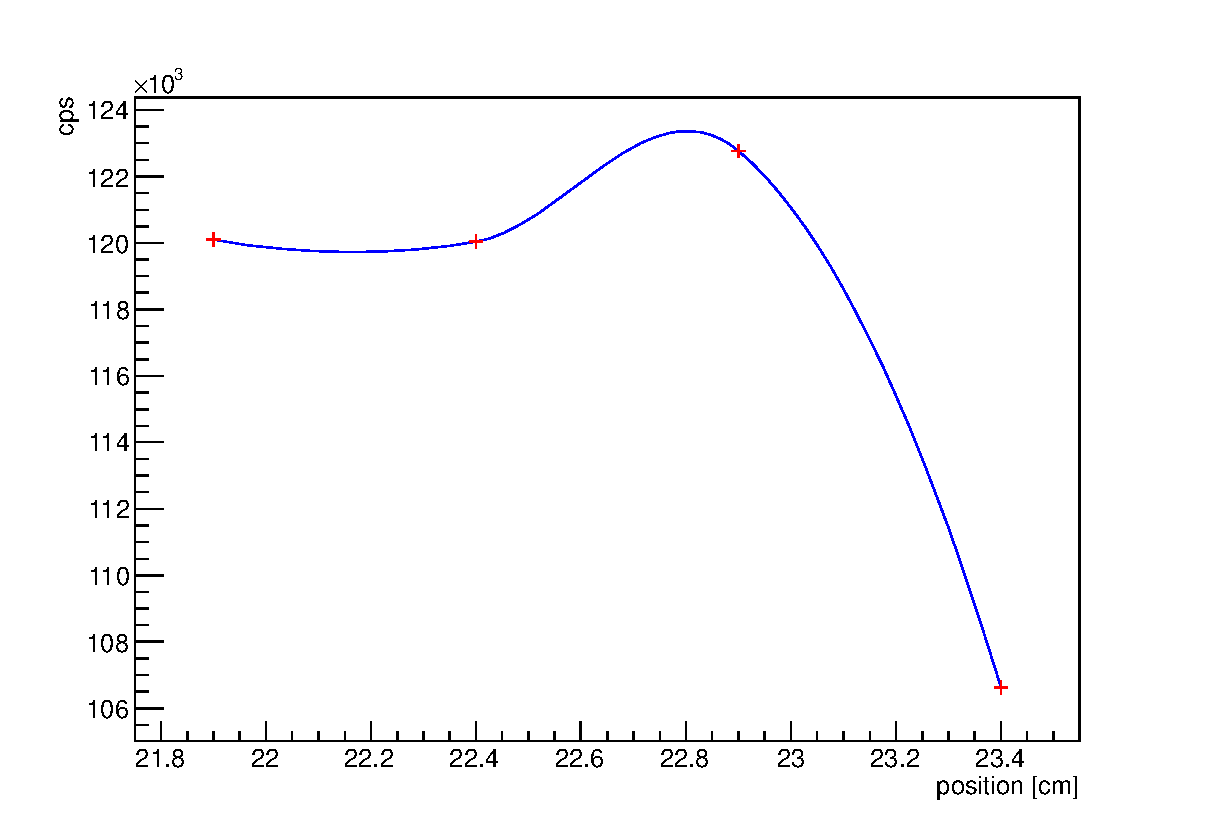
\includegraphics[width=\textwidth]{graphics/cobalt/modules/8B.eps}
	\end{minipage}
	
	
  	%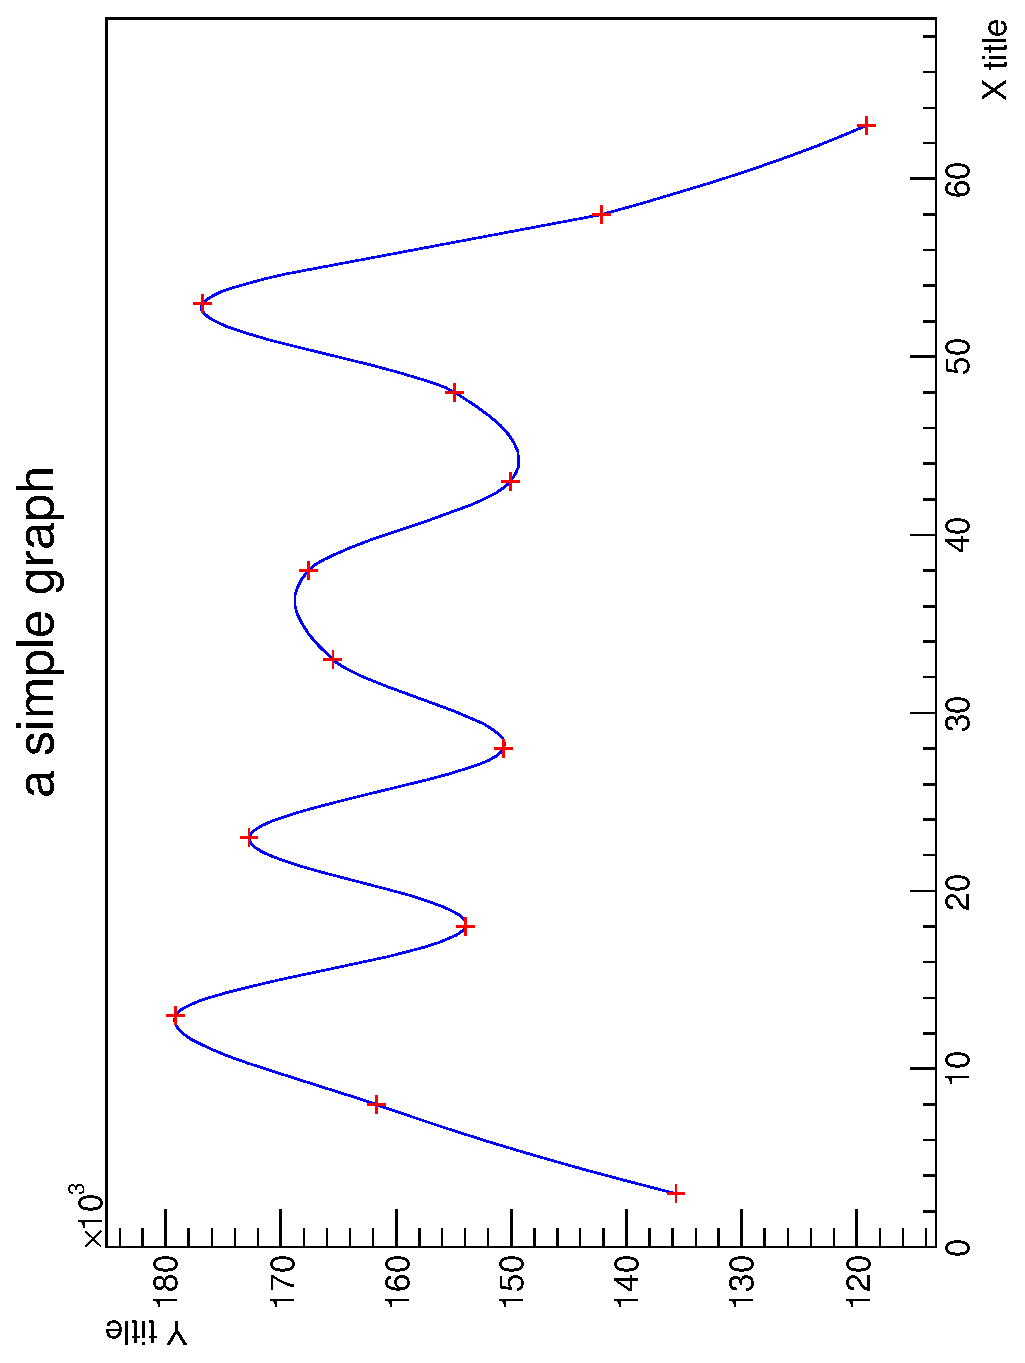
\includegraphics[angle = -90, width = 0.9 \textwidth]{graphics/cobalt/876_parallel_good.eps}
  	\caption[Testing of all modules with cobalt source]{Measurements with source at different positions}
  	\label{fig:SrRatesPMT}
  \end{figure}

    %% ===========================
  \section{Synchronisation of moun module and FPD DAQs}
  \label{ch:Analysis:sec:Synchronisation of moun module and FPD DAQs}
  %% ===========================  
  Measuring time differences on a \SI{}{\micro\second} scale requires exact synchronisation of the two differen DAQs used for data acquisition. For this purpose, a clock has been designed sending signals at two frequencies: one at \SI{1}{\hertz} and one at \SI{10e6}{\hertz} internally converted to a \SI{20 e 6}{\hertz} signal by the DAQ. Those signals can be synchronised to the timestamps of GPS satellites if a GPS antenna is connected. This has not yet been done as relative synchronization between the two crates is sufficient for the purposes of finding correlations between muon and detector events. As the cable length for signal transmission is pretty extensive - around \SI{50}{\meter} - it was decided to use optical fibers instead of CAT 5 cabling. As two signals need to be transmitted, paired \todo{connection type name} fibers were used. The clock itself has optical outputs, the DAQ though needs converters from optical to electrical signals and a modified SLT back panel card to receive the converted 
signals via Cat 5 cable.
  \begin{figure}
  	
\includegraphics[width = 0.9 \textwidth]{graphics/dummy.eps}
  \end{figure}

  
  To test the setup, the muon DAQ was moved to the detector platform. Both crates were fed by a pulser signal. Runs at different frequencies were recorded to test both the synchronisation and the detection of events. To synchronize timestamps to an external signal, the FLT cards drop down menu needs to be set to \todo{look up} and the SLT needs to be set to \todo{lookup too}.
  At first, manually triggered signals were used in minute runs to check the timestamps equality. Several runs were taken, all showing that the events were shifted by several \SI{}{\micro\second}
  \begin{figure}
  	
\includegraphics[width = 0.9 \textwidth]{graphics/dummy.eps}
  	\caption[Synchronisation old firmware]{Subsecond time differences before firmware update: Large differences between the events, }
  \end{figure}

  In close cooperation with the IPE it was found that this was merely a problem of firmware versioning as well as software settings in Orca resolving the problem quickly. After installing the latest firmware, more runs were taken now displaying the desired behaviour:
  \begin{figure}
	\caption[Synchronisation new firmware]{Time differences between events after firmware upgrades. Differences between the event times are within one \SI{50}{\nano\second} bin}
  	
\includegraphics[width = 0.9 \textwidth]{graphics/dummy.eps}
  \end{figure}
  Following the manually triggered events, runs with fixed frequency events were recorded, raising the frequency to up to \todo{find maximum}. All the test worked fine including starting one DAQ's run way ahead of the other. Those events recorded in both run files were always well synchronized.
  Afterwards, the muon DAQ was moved back to its original position and the optical fibers were stowed in wire-ways guiding it from the detector platform down to the basement where the muon detection system is located. Another problem occurred here, as signal transmission was impaired by a kink at one of the turns, but was quickly resolved by smooth rewiring.
  Concluding, it can be said that the clock runs continuously without any problems throughout all the measurements - including main spectrometer commissioning measurements.

  
  %% ===========================
  \section{Coincidence Search between Muon- and Detector Events}
  \label{ch:Analysis:sec:Monitor Spectrometer Measurements}
  %% ===========================  
  If one wants to actually detect background induced by myonic events registered by the muon modules, those events need to be correlated to detector events time wise. For this purpose, the analysis code's class run was extended by the member functions TOFHist()\ref{ch:Analysis software:sec:methods of the class run:subsec:TOFHist()} and TOFMuonDet()\ref{ch:Analysis software:sec:methods of the class run:subsec:TOFMuonDet()}, where the former is used for monitor spectrometer analysis and the latter for the main spectrometer. The biggest difference is that, at the main spectrometer, two DAQs leading to runs with different starting times and of different lengths are created that need to be compared. 
  
  %% =========================
  \subsection{Monitor Spectrometer}
  \label{ch:Analysis:sec:Monitor Spectrometer Measurements:subsec:Monitor Spectrometer}
  %% =========================
  
  Measurements at the monitor spectrometer are easily manageable due to the fast accessibility of all the components and the collection of data in a single run file through the mini crate.
  For measurements, high voltage supplies have been added to the \todo{name of the rack} rack and the readout electronics were connected to a second FLT-card inserted into the mini DAQ and operated in veto mode. Gains and thresholds were easily set as only four sides had to be adjusted - compared to the 16 main spectrometer channels. The PMT tubes were operated at \SI{1.5}{\kilo\volt}. The detector gain and threshold settings for the 5 pixel detector have been kept, although the detector position has been shifted to the position at which the center pixel exhibited maximum rate and the pairs of east-west and top-bottom pixels showed comparable count rates. Furthermore, the recording mode was switched from histogram mode to energy mode as the timestamps for every single event were needed for analysis. 
  Several hourly runs have been taken under different magnetic field compositions. Both asymmetric magnetic field (see table \ref{tab:analysis:asymmetricMagneticFields} and figure \ref{fig:monSpec:asymmetric magnetic field} and non-axially-symmetric field (see table \ref{tab:analysis:nonAxiallySymmetricField} and figure \ref{fig:monSpec:non axially symmetric magnetic field} configurations have been investigated. \todo{}
  \begin{table}
	\centering
		\begin{tabular}{c}
		\end{tabular}\\
		\begin{tabular}{|l|ccccccc|}
			\hline
			\centering
			
			Run &  solenoid &solenoid &inner & outer &outer &emcs x	&emcs y\\
			& 	source	& detector & aircoil & central aircoil & aircoil& &\\
			\hline
			mos00159395& 0&	25&	0&	-4&	-4&	2&	-19.5\\
			\hline
			mos00159396-&&&&&&&\\
			mos00159398 & 0 & 50& 0 & -8 & -8 & 2 & -19.5\\
			mos00159399 & 0 & 50& 0 & -7 & -7 & 2 & -19.5\\
			\hline
			mos00159400 & 0 & 50& 0 & -6 & -6 & 2 & -19.5\\
			\hline
			mos00159401 & 0 & 10& 0 & -2 & -2 & 2 & -19.5\\
			\hline
			mos00160713-&&&&&&&\\
			mos00160717& 0.1 & 12.5 & 0 & -2 & -2 & 0 & 0\\
			\hline
			mos00160718-&&&&&&&\\
			mos00160730 & 0.1 & 12.5 & 0 & -2 & -2 & 0 & 0\\
			\hline
			mos00161105-&&&&&&&\\
			mos00161107 & 0.1 & 12.5 & 0 & -2 & -2 & 0 & 0\\
			\hline
			mos00161108-&&&&&&&\\
			mos00161110 & 0.1 & 25 & 0 & -2 & -2 & 0 & 0\\
			\hline
		\end{tabular}
		\caption[Asymmetric magnetic field measurements]{Measurements at asymmetric magnetic fields. The source side magnet was turned off for all measurements leaving the flux tube entering the spectrometer walls.}
		\label{tab:analysis:asymmetricMagneticFields}
	\end{table}
	\begin{table}
		\begin{tabularx}{\textwidth}{|L{1.1cm}|>{\centering}X|>{\centering}X>{\centering}X>{\centering}X>{\centering}X>{\centering}X>{\centering}X>{\centering\arraybackslash}X|}
			\hline
			\parbox[t]{2mm}{\multirow{3}{*}{\rotatebox[origin=c]{90}{ Run mos00... }}}
			&\parbox[t]{2mm}{\multirow{3}{*}{\rotatebox[origin=c]{90}{\bf 2 Horizontal loops }}}
			&\parbox[t]{2mm}{\multirow{3}{*}{\rotatebox[origin=c]{90}{solenoid source }}}
			&\parbox[t]{2mm}{\multirow{3}{*}{\rotatebox[origin=c]{90}{solenoid detector }}}
			&\parbox[t]{2mm}{\multirow{3}{*}{\rotatebox[origin=c]{90}{inner aircoil }}}
			&\parbox[t]{2mm}{\multirow{3}{*}{\rotatebox[origin=c]{90}{ outer aircoil }}} 
			&\parbox[t]{2mm}{\multirow{3}{*}{\rotatebox[origin=c]{90}{outer cent. aircoil }}}
			&\parbox[t]{2mm}{\multirow{3}{*}{\rotatebox[origin=c]{90}{EMCS x }}}
			&\parbox[t]{2mm}{\multirow{3}{*}{\rotatebox[origin=c]{90}{EMCS y }}}\\
			
			
			
			&&&&&&&&\\
			&&&&&&&&\\
			&&&&&&&&\\
			&&&&&&&&\\
			&&&&&&&&\\
			&&&&&&&&\\
			&&&&&&&&\\
			\hline
			161111-161125 & 0 & 25 & 25 & 6.8 & 7 & 5 & 0 & -14\\
			\hline
			161126-161129 & +50 & 12.5 & 12.5 & 3.5 & -3.5 & 2.5 & 0 & 0\\
			\hline
			161130-161133 & +25 & 12.5 & 12.5 & 1.75 & -1.75 & 1.25 & 0 & 0\\
			\hline
			161134-161149 & -25 & 12.5 & 12.5 & 1.75 & -1.75 & 1.25 & 0 & 0\\
			\hline
			161150-161155 & -50 & 12.5 & 12.5 & 3.5 & -3.5 & 2.5 & 0 & 0\\
			\hline
			161156-161158 & 0 & 12.5 & 12.5 & 3.5 & -3.5 & 2.5 & 0 & 0\\
			\hline

			
			\hline
		\end{tabularx}
		\caption[Non axially-symmetric magnetic field measurements]{Measurements in energy mode at non axially symmetric magnetic field. Both solenoid and air coil currents have bee changed, though always by a multiplication factor for all of them so that the ration remained the same.}
		\label{tab:analysis:nonAxiallySymmetricField}
		
  	\end{table}
  	
  	
  The TOFHist\ref{ch:Analysis software:sec:methods of the class run:subsec:TOFHist()} function has been used to analyse the data.
  It browses through all the muon events detected and finds any detector event in a definable timespan after the muon event. This can be more than one detector event per  muon event. In all of the settings, a clear peak is visible at around \SI{7}{\micro\second}. As for count rates, they are a lot higher in the asymmetric magnetic field setup as secondary electrons are guided from their point of origin to the detector instead of mostly being magnetically shielded. In this setup, only the reflection through the rise in magnetic field on the electrons' paths takes its toll on the rate.
  A graphic of the flux tube configuration as well as the histograms for all of the settings can be found in the \ref{appendix}, figures \todo{reference figures.}
  The exact values are:
  \begin{table}
  	\begin{tabularx}{0.8\textwidth}{>{\centering}X>{\centering\arraybackslash}X}
  		Average & Standard Deviation\\
  	\end{tabularx}
  \end{table}

  \todo{Do analysis for every measurement, insert peak positions + stdev}
  
  
  \begin{figure}
	
\includegraphics{graphics/dummy.eps}
	\caption[Asymmetric magnetic field flux tube]{Flux tube at asymmetric magnetic fields. Electrons from processes at the walls are guided directly towards the detector as the largest part of the flux tubes surface ends in the monitor spectrometer's vessel's wall}
  	\label{fig:monSpec:asymmetric magnetic field}
  \end{figure}

    \begin{figure}
	
	
\includegraphics{graphics/dummy.eps}
  	\caption[Non-axially symmetric magnetic flux tube]{Flux tube at non axially symmetric fields. Although no direct guidance from the wall to the detector is given (the flux tube never touches the wall in this configuration), by adding a magnetic component perpendicular to z-direction, the probability for entrance into the flux tube rises strongly.}
  	\label{fig:monSpec:non axially symmetric magnetic field}
  \end{figure}
  
  \begin{figure}
	\label{fig:monSpec:timeDifferences asymmetric magnetic field}
	\caption[Time difference histogram]{Time difference histogram for asymmetric magnetic fields.}
  	
\includegraphics{graphics/dummy.eps}
  \end{figure}
  
  \begin{figure}
	\label{fig:monSpec:timeDifferences non axially symmetric magnetic field}
	\caption[Non-axially symmetric magnetic flux tube monitor spectrometer]{Flux tube at non axially symmetric fields. Although no direct guidance from the wall to the detector is given (the flux tube never touches the wall in this configuration), by adding a magnetic component perpendicular to z-direction, the probability for entrance into the flux tube rises strongly.}
  	
\includegraphics{graphics/dummy.eps}
  \end{figure}  
  %% =========================
  \subsection{Main Spectrometer}
  \label{ch:Analysis:sec:Monitor Spectrometer Measurements:subsec:Main Spectrometer}
  %% =========================
  
  Monitor spectrometer results suggested that the time of flight was well measurable, even if on bigger scale, at the main spectrometer. So, during commissioning measurements, already parallel to measurement M1, sone runs with asymmetric magnetic field have been taken with switched polarity or turned off pre spectrometer magnets compared to standard setup.
  The data was analysed for each single ring of the FPD. Search parameters were the time slot from \SI{0}{\second} to \SI{15}{\micro\second} though remains inconclusive at the moment, see \ref{fig:mainSpec:allRings}. Analysis for every single pixel was not possible due to much too low statistics, though it might be more conclusive as less different paths contibute to the single pixel. On the other hand, after the non-central alignment of the detetor has been fixed using different settings for the LFCS-system, under asymmetric magnetic fields, the fields should be rotationally symmetric around the z axis disregarding small deviations. Assuming this, the path lengths for every pixel of one ring should be very comparable.
  
  \begin{figure}
  \centering
  	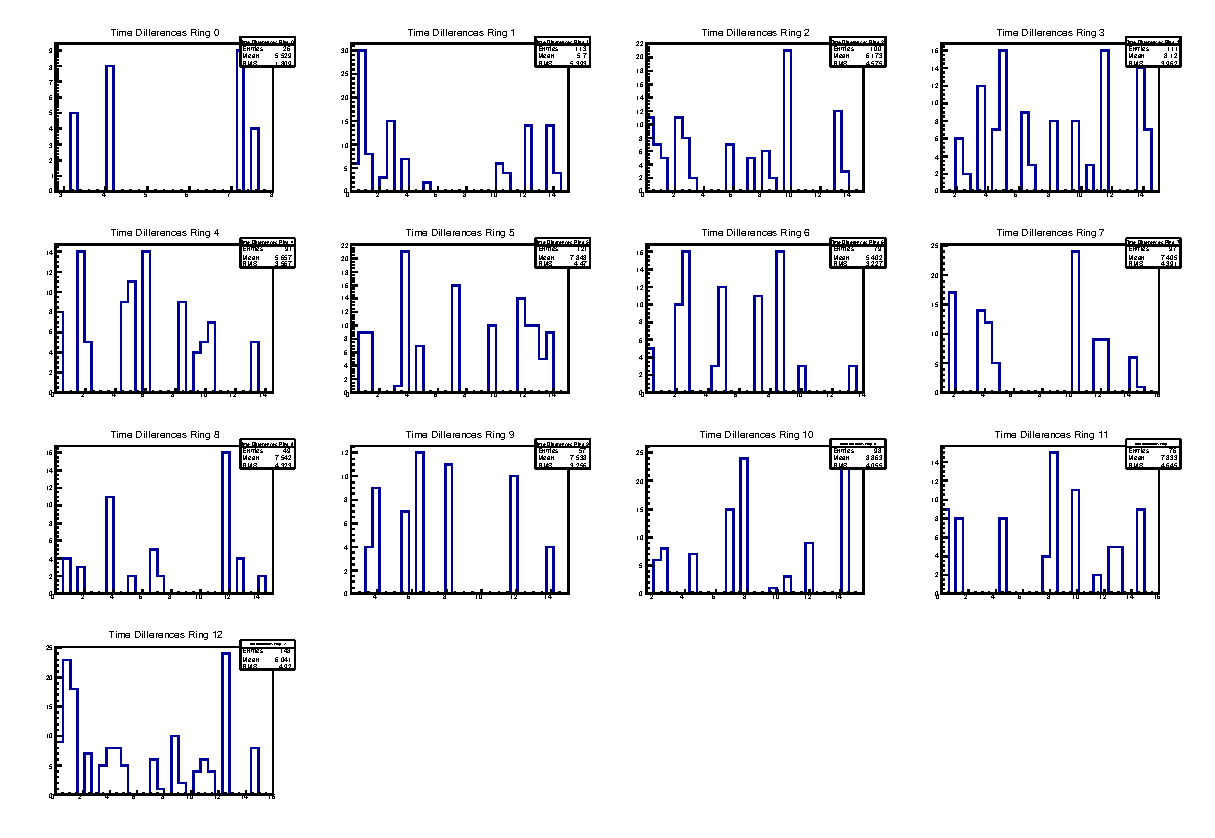
\includegraphics[width = 0.9 \textwidth]{graphics/mainSpec/mainSpecRings.eps}
  	\caption[Time difference Histogram for all rings]{Time differences of muon events followed by a detector event. From left to right and top down for every single detector ring, 0 being the innermost and 12 being the outermost ring.}
  	\label{fig:mainSpec:allRings}
  \end{figure}

  
  The failure to find a clear runtime for electrons induced by muonic events might be due to the combination of muon module position and the magnetic field setup as the wall area covered by the flux tubes and the volume surveilled by the muon modules did not overlap very much. Furthermore, due to the very low magnetic field at the wall compared to the volume inside the detector and pinch magnet, most of the induced electrons are magnetically reflected as the maximum polar angle towards magnetic field lines $\theta_{max}$ is defined by
  \begin{equation}
  	\frac{B_{min}}{B_{max}} \approx \frac{\SI{3}{\gauss}}{\SI{4}{\tesla}} = sin(\theta_{max})
  \end{equation}
  meaning only angles satisfying the inequation
  \begin{equation}
  	\theta < \arcsin{\frac{B_{min}}{B_{max}}} = \arcsin{\frac{\SI{3}{\gauss}}{\SI{4}{\tesla}}} = \SI{0.004}{\degree}
  \end{equation}
  will be able to reach the detector. All others will be reflected and fly back to the wall to be absorbed in the conducting wall material. \todo{set real field values}
  As a result, compared to the monitor spectrometer, where the ratio is a lot greater, less of the muon induced electrons arrive at the detector making long measurements a requirement for good statistics. This leads to detector rates of only around \SI{2}{\cps}, depending on the inner electrode voltages. At high inner electrode voltages, the rate increases strongly to \SI{150}{\cps} which is probably due to field emission from the electrodes. 
  These measurements should be repeated when high voltage can be applied to the main vessel.

  
    Following that presumption, for M6 measurements, the setup was changed. The fluxtube was widened for its outer parts to hit the spectrometer wall in regions around combs n and n \todo{which combs}. This raises the probability of the muons detected being those inducing secondary electrons at the vessel as well. Also, the LFCS setup was changed in such fashion that the magnetic field at the spectrometer wall is higer by a factor of two, directly resulting in a higher angular acceptance of electrons. The resulting flux tube is shown in figure \ref{fig:newFluxTube}. 
    
    
  \todo{flux tube including modules for horizontal and vertical view}
  \begin{figure}
	
\includegraphics[width = 0.9 \textwidth]{graphics/dummy.eps}
	\caption[Flux tube P12.M8]{New flux tube}
  	\label{fig:newFluxTube}
  \end{figure}
  \todo{If data will be taken add to analysis.}
  
  \begin{figure}
	\caption[Flux tube M12.8]{Flux tube in field configuration M12.8}
  	
\includegraphics[width = 0.9 \textwidth]{graphics/dummy.eps}
  \end{figure}
  
  \begin{figure}
  	\caption[Inner electrode field emission]{Rate trend over inner electrode voltages}
  	
\includegraphics[width = 0.9 \textwidth]{graphics/dummy.eps}
  \end{figure}

  

  
  
